% =====================================================================
%  Aerial Cetacean Detection across the Ground-Sample-Distance Axis
%  Technical report / paper -- SurveyLabs, AEROSUB (HORIZON-EU 101189723)
%
%  Compile:  ./build.sh        (uses the bundled tectonic in .tools/)
%  Format:   single-column `article` for easy editing. To reformat for a
%            journal (IEEEtran / MDPI / elsarticle) swap \documentclass and
%            the bibliography style -- body text is class-agnostic.
% =====================================================================
\documentclass[11pt,a4paper]{article}

\usepackage[utf8]{inputenc}
\usepackage[T1]{fontenc}
\usepackage{lmodern}
\usepackage[margin=1in]{geometry}
\usepackage{graphicx}
\usepackage{booktabs}
\usepackage{amsmath,amssymb}
\usepackage{subcaption}
\usepackage{caption}
\usepackage{xcolor}
\usepackage{enumitem}
\usepackage{authblk}
\usepackage[numbers,sort&compress]{natbib}
\usepackage{tikz}
\usetikzlibrary{arrows.meta,positioning,shapes.geometric}
\usepackage{microtype}
\usepackage{xurl}
\usepackage{etoolbox}
\usepackage[section]{placeins}
\usepackage{float}
% Let floats fill more of each page so they are not deferred (less whitespace).
\setcounter{topnumber}{4}
\setcounter{bottomnumber}{4}
\setcounter{totalnumber}{8}
\renewcommand{\topfraction}{0.95}
\renewcommand{\bottomfraction}{0.95}
\renewcommand{\textfraction}{0.05}
\renewcommand{\floatpagefraction}{0.85}
\usepackage[hidelinks]{hyperref}
\captionsetup{font=footnotesize,labelfont=bf}

\definecolor{slblue}{RGB}{0,90,140}
\newcommand{\todo}[1]{\textcolor{red}{[TODO: #1]}}
\newcommand{\map}{mAP}
\newcommand{\imgsz}{1024}
\newcommand{\fppi}{\text{FPPI}}

\setlength{\emergencystretch}{3em}

\title{\bfseries Aerial Cetacean Detection for Autonomous Offshore
Monitoring: One Detector across the Ground-Sample-Distance Axis, from
Exact Detection to Wide-Area Screening}

\author[1]{Gerard Dooly}
\author[1]{Petar Trslic}
\affil[1]{SurveyLabs Ltd., Ireland \\ \texttt{\{gerard.dooly, petar.trslic\}@surveylabs.ie}}

\date{\today}

% ---------------------------------------------------------------------
\begin{document}
\maketitle

\begin{center}\small\itshape
Technical report --- work in progress. Data sources, the detector and the
reported results are updated as the AEROSUB project progresses.
\end{center}

\begin{abstract}
Environmental monitoring of cetaceans around offshore-wind developments is
labour-intensive, relying on trained observers and slow manual review of survey
imagery. As part of the HORIZON~Europe project \textbf{AEROSUB}
(GA~101189723), SurveyLabs is developing an autonomous aerial monitoring
capability in which a long-range vertical take-off and landing (VTOL)
fixed-wing UAS detects cetaceans over open water. This report documents the
RGB perception component. We first consolidate ten heterogeneous aerial and
near-surface sources into a unified, deduplicated dataset of $27{,}290$~images
/ $55{,}163$~annotations through a reproducible normalisation pipeline that
fixes label-format, EXIF-orientation and offline-augmentation inconsistencies,
and we describe a Label~Studio human-in-the-loop pseudo-labelling loop for
growing it. Our organising argument is that a single aerial detector is
asked to operate across a wide \emph{ground-sample-distance} (GSD) axis, and
that the two ends of that axis are two different tasks: at \emph{high} GSD the
animal is resolved to hundreds of pixels and the task is \emph{exact
detection} (localise and count), whereas at \emph{low} GSD the animal collapses
to a few pixels and the only realistic task is \emph{wide-area screening} ---
cueing a human expert at high recall for a small false-alarm budget. A six-way controlled study
(varying backbone capacity, data composition and hard-negative dose one factor
at a time) shows that low-GSD screening recall is governed by data composition
and capacity rather than tuning: removing the porpoise source collapses the
detector, extra surface data hurts, and --- reversing a common assumption ---
the larger \textbf{YOLO11s} backbone lifts screening recall substantially
($0.535$ vs $0.412$ recall at $1$~false positive per image) even though it
barely moves precision-regime \map. We then introduce \textbf{adaptive SAHI}, a
telemetry-driven slicing scheme that ties tile size to GSD so the detector
sees animals at a roughly consistent apparent scale. In a single-frame
illustration on a real $151$-megapixel survey frame, plain whole-frame inference
detects \emph{none} of three resolvable dolphins whereas adaptive SAHI recovers
all three with zero false positives at $17\times$ fewer tiles than the best fixed
slice; a semi-synthetic altitude sweep shows the same policy holding recall
comparable to fixed slicing while spending tiles only as geometry demands.
Finally we quantify the practical limit of the low-GSD end: on out-of-domain
survey frames the detector plateaus near $0.6$ recall at $2$ false positives per
image --- useful triage, but a real domain gap that further in-domain
pseudo-labelling is designed to close. The
model, data pipeline and inference tooling form the basis of AEROSUB
deliverable D2.1 and key exploitable result KER9.
\end{abstract}

\noindent\textbf{Keywords:} cetacean detection, aerial imagery, UAS, YOLO,
small-object detection, SAHI, ground-sample distance, offshore wind, marine
mammal monitoring.

% =====================================================================
\section{Introduction}
% =====================================================================
Offshore wind is expanding rapidly, and with it the regulatory requirement to
monitor the impact of construction and operation on marine megafauna.
Cetaceans (whales, dolphins and porpoises) are protected species whose presence
must be assessed before and during noisy activities such as pile driving.
Present practice relies on \emph{marine mammal observers} stationed on vessels
or platforms, and on manual review of aerial or vessel survey imagery. This is
expensive, weather-limited, spatially restricted, and slow: latency from image
capture to a confirmed sighting can be tens of minutes.

Within the HORIZON~Europe project \textbf{AEROSUB} (Grant Agreement
101189723), SurveyLabs is tasked with on-board \emph{detection and tracking} of
cetaceans from RGB aerial imagery. This report documents that work: a robust
aerial cetacean detector, the data pipeline that feeds it, and the survey-scale
inference machinery around it.

\paragraph{Central argument: one detector, one GSD axis, two tasks.}
The organising thesis of this report is that open-water detection reliability
is governed less by raw model capacity than by \emph{data composition} and
\emph{scale-aware inference}, and that these two levers act at opposite ends of
a single continuum --- the \textbf{ground-sample distance} (GSD, metres of
water per image pixel) at which an animal is imaged. A survey aircraft does not
fly at one scale: altitude, lens and sensor set how many pixels a given animal
subtends, and that number spans orders of magnitude across a campaign. We argue
that the two ends of this GSD axis are not the same problem measured more or
less precisely --- they are \emph{different tasks} that deserve different
metrics:
\begin{itemize}[itemsep=2pt,topsep=2pt]
  \item \textbf{High-GSD, exact-detection regime.} When the animal is resolved
  to hundreds of pixels (low altitude, high-resolution sensor, or
  scale-recovered by tiling), the operational task is to localise and count
  individual animals. The right metric is precision and mean average precision
  (\map) against exact ground-truth boxes. The real anchor for this regime is a
  $151$-megapixel survey frame at GSD~$\approx\!2.4$~cm/px
  (Section~\ref{sec:apem}), where scale-aware inference recovers the full pod.
  \item \textbf{Low-GSD, screening regime.} When the animal collapses to a
  handful of pixels (high altitude, coarse GSD, or a foreign survey domain),
  exact localisation is neither achievable nor the objective. The only realistic task
  is \emph{screening}: flag frames that plausibly contain an animal at high
  recall for a small false-alarm budget, so a human expert reviews a short
  queue instead of the whole flight. The right metric is recall at a fixed
  number of false positives per image (recall@$\fppi$, an FROC curve). The real
  anchor here is an out-of-domain aerial marine-mammal survey
  (Section~\ref{sec:screening}), where the detector reaches useful but bounded
  triage recall.
\end{itemize}

\paragraph{In plain terms: two axes, five tests.} Two things change
independently in an aerial survey, and conflating them is the usual source of
misleading accuracy numbers. The first is \emph{scale} --- how many pixels the
animal actually spans, set by altitude and sensor rather than by the animal
itself. The second is \emph{domain} --- whether a frame \emph{looks like} the
imagery the detector was trained on (same style of sensor, sea state and
viewpoint) or comes from a different survey it has never seen. Every experiment
in this report is deliberately one cell of the resulting $2\times2$ ---
scale (resolved vs.\ a few pixels) $\times$ domain (in-distribution vs.\ a
foreign survey) --- each chosen to isolate a single effect. Table~\ref{tab:roadmap}
places all of them on both axes at once, so the reader does not have to reassemble
the picture from scattered sections: it separates what tiling \emph{can} fix (a
\emph{scale} problem) from what it cannot (a \emph{domain} problem).

The same trained weights serve both ends; what changes along the axis is the
\emph{inference geometry} (Section~\ref{sec:inference}) and the appropriate criterion
by which success is judged. Every component below supports this claim: the
curation pipeline controls what the detector learns
(Section~\ref{sec:data}); a controlled six-way study isolates which
data/capacity choices move the low-GSD screening floor
(Section~\ref{sec:screening}); adaptive SAHI restores the high-GSD exact-detection
regime a fixed model cannot reach (Section~\ref{sec:inference}); and an explicit
discussion of the domain gap (Section~\ref{sec:gap}) bounds what the low-GSD end
can promise today.

\paragraph{Contributions.} This report makes the following contributions:
\begin{enumerate}[itemsep=2pt,topsep=2pt]
  \item A reproducible \textbf{data-curation pipeline}
  (Section~\ref{sec:data}) that unifies ten heterogeneous public
  aerial and surface sources into a single deduplicated dataset, resolving
  label-format, EXIF-orientation and offline-augmentation pitfalls that
  silently corrupt naively merged training sets, plus a Label~Studio
  human-in-the-loop pseudo-labelling loop for dataset growth.
  \item A framing of the deployment problem as a \textbf{GSD axis with two
  tasks and two metrics} (exact detection via \map; screening via
  recall@$\fppi$), and a \textbf{controlled six-way study}
  (Section~\ref{sec:screening}) that isolates the effect of backbone capacity,
  surface data, the porpoise source and hard-negative dose on each --- showing
  that composition and capacity, not tuning, govern the low-GSD screening
  floor.
  \item \textbf{Adaptive SAHI} (Section~\ref{sec:inference}), a telemetry-driven
  slicing scheme that couples tile size to GSD so the detector observes animals
  at a consistent apparent scale, with a fall-back cascade for missing
  metadata, validated on a semi-synthetic altitude sweep and on a real
  $151$-megapixel survey frame.
  \item An explicit \textbf{domain-gap analysis} (Section~\ref{sec:gap}) that
  separates the pure GSD effect (isolated on synthetic data) from the
  domain-shift effect (a foreign real survey), and states the resulting recall
  ceiling as an explicit limitation.
  \item A \textbf{ROS~2 deployment node} (Section~\ref{sec:ros}) that runs the
  detector on live or replayed imagery under a selectable inference strategy
  (fixed, adaptive or adaptive-range), reusing the exact offline inference core
  and publishing standard \texttt{vision\_msgs} detections into the AEROSUB
  autonomy stack.
\end{enumerate}

\begin{table}[ht]
\centering
\caption{\textbf{Experimental roadmap.} Every evaluation in this report placed on
both axes at once. \emph{Scale} = how many pixels the animal spans (set by
altitude and sensor); \emph{Domain} = in-distribution vs.\ a foreign survey the
detector was not trained on. Reading them together separates the \emph{scale}
effect (addressed by adaptive SAHI, Section~\ref{sec:inference}) from the residual
\emph{domain} gap (addressed by in-domain pseudo-labelling, Section~\ref{sec:gap}).}
\label{tab:roadmap}
\footnotesize
\setlength{\tabcolsep}{4pt}
\renewcommand{\arraystretch}{1.15}
\begin{tabular}{@{}llllp{4.2cm}@{}}
\toprule
\textbf{Test set} & \textbf{Scale} & \textbf{Domain} & \textbf{Task / metric} & \textbf{What it isolates} \\
\midrule
Aerial slice & resolved & in-dist. & exact / \map & ceiling when nothing shifts ($\map50\ 0.82$--$0.86$) \\
\texttt{whale-bbox-layer} & resolved & \textbf{foreign} & exact / \map & pure \textbf{domain} gap; SAHI cannot help ($\map50\ 0.54$) \\
Synthetic sweep & varied & in-dist. & recall / tiles & pure \textbf{scale} effect --- adaptive SAHI's job \\
HiDef survey & tiny & \textbf{foreign} & screening / recall@$\fppi$ & scale $+$ domain together ($\approx\!0.6$ ceiling) \\
APEM frame & tiny$\to$resolved & \textbf{foreign} & exact / TP--FP & SAHI restores scale ($3/3$) \\
\bottomrule
\end{tabular}

\vspace{3pt}
{\footnotesize\emph{Scale is the solved axis (adaptive SAHI); domain is the
residual ceiling (pseudo-labelling).}}
\end{table}

% =====================================================================
\section{Related Work}
% =====================================================================
\paragraph{Aerial marine-mammal detection.}
Automated detection of marine mammals in aerial imagery has been explored with
classical and deep approaches
\citep{maire2015beach,hodgson2013uav,gray2019drones,boulent2023detecting,corrigan2014aerial}.
Early systems used hand-crafted features and sliding windows; recent work uses
CNN detectors on drone and manned-survey imagery. The recurring difficulties
are extreme scale variation of targets (from a few pixels to a large fraction
of the frame), confusion with sun glint, whitecaps and wakes, and the scarcity
of labelled data --- all of which we observe and address here.

\paragraph{Digital aerial surveys and the GSD ceiling.}
The operational context for this work is the \emph{digital aerial survey}, now
the standard method for offshore-wind wildlife baselines in the UK and Ireland.
Two commercial providers dominate this market: HiDef Aerial Surveying
Ltd.\footnote{\url{https://www.hidefsurveying.co.uk/}} flies high-altitude
digital video and stills tuned for wide-area \emph{screening}, while
APEM Ltd.\footnote{\url{https://www.apemltd.com/}} operates very-high-resolution
still cameras (Phase~One medium format) cited as a UK benchmark for survey
design. The two providers sit at opposite ends of the ground-sample-distance
(GSD) axis that organises this paper --- HiDef anchoring the low-GSD screening
regime and an APEM-class $151$-megapixel frame anchoring the high-GSD
exact-detection regime (Section~\ref{sec:inference}). \citet{bartlett2025offshore},
whose authors include members of the present team, report that at the GSD
typical of such surveys an individual animal spans only a handful of pixels, so
that automated pipelines are well suited to detecting and counting animals but
exact species-level identification from a single frame is inherently limited ---
precisely the two-task, two-metric split we adopt here.

\paragraph{One-stage detectors.}
The YOLO family \citep{redmon2016yolo,ultralytics2023yolo} provides real-time
single-stage detection suitable for on-board deployment. We use YOLO11
\citep{khanam2024yolov11}; unlike much prior work that fixes on the smallest
backbone for edge speed, we treat backbone capacity as an experimental variable
(Section~\ref{sec:screening}) and find it matters specifically for the low-GSD
screening regime.

\paragraph{Small-object and screening inference.}
Survey frames are tens to hundreds of megapixels, but detectors ingest a fixed,
much smaller input; naive downscaling destroys small targets. Slicing-Aided
Hyper Inference (SAHI) \citep{akyon2022sahi} runs the detector on overlapping
tiles and merges results, trading compute for recall on small objects. We build
on SAHI and extend it with telemetry-driven tile sizing
(Section~\ref{sec:inference}). For video, multi-object tracking \citep{aharon2022botsort}
stabilises detections. Because the low-GSD regime is a detection/screening task
with a small target set and a tolerance for coarse localisation, we score it
with a free-response operating characteristic (FROC): recall against false
positives per image, a standard screening metric, rather than \map{} alone.

% =====================================================================
\section{Data, Curation, Labelling}\label{sec:data}
% =====================================================================
\subsection{Sources}
We aggregate ten datasets confirmed to contain only cetacean targets, spanning
nadir and oblique aerial views and near-surface imagery
(Table~\ref{tab:sources}). Sources arrive in incompatible formats:
Roboflow-YOLO exports, plain per-scene YOLO text files, VIA polygon JSON (the
Dryad humpback/blue-whale set), and NOAA-style sighting CSVs. Species range
from large whales that fill much of the frame to porpoises only a few pixels
across, giving a demanding multi-scale detection problem
(Fig.~\ref{fig:corpus}). All annotations are
collapsed to a single class (\texttt{cetacean}).

\begin{figure}[ht]
\centering
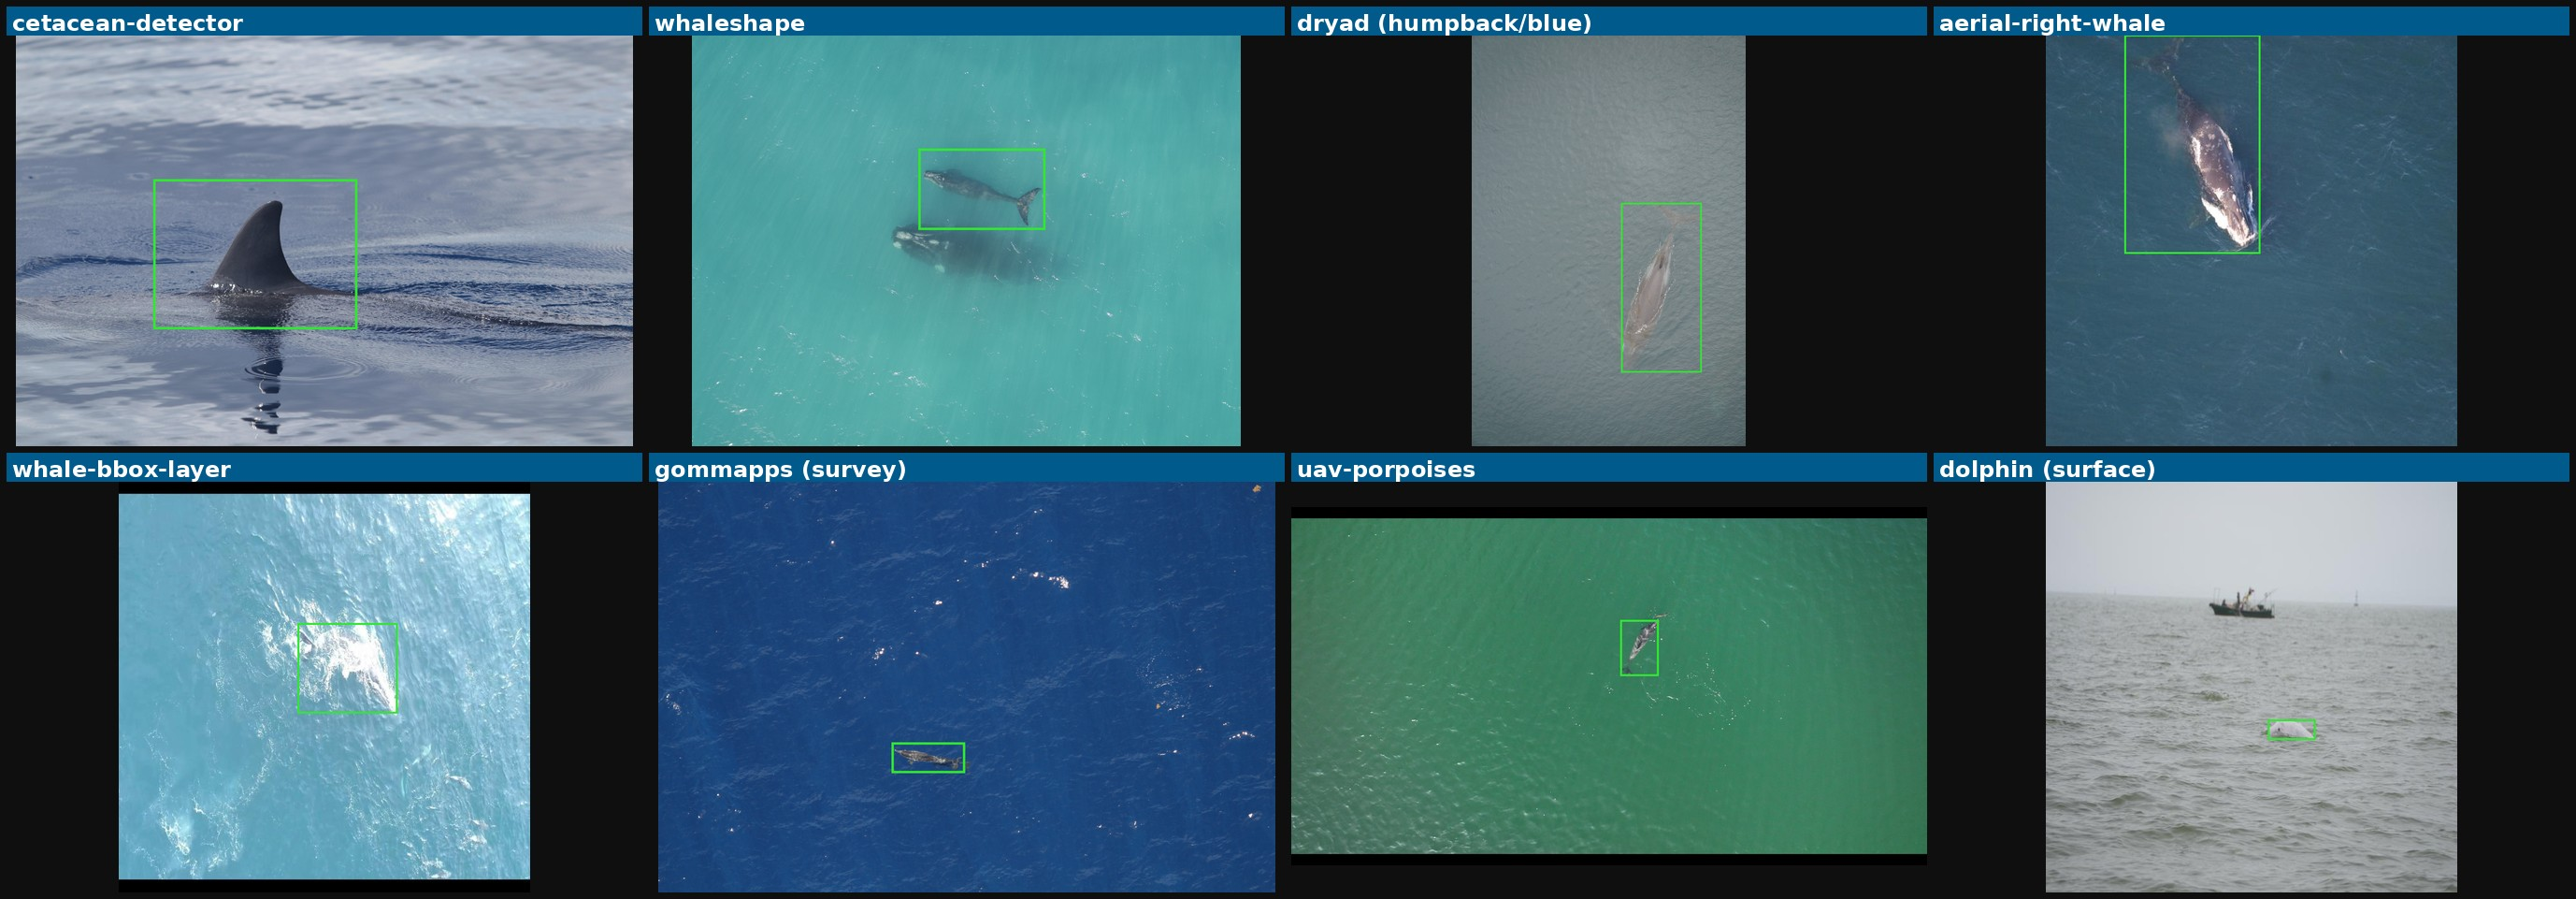
\includegraphics[width=\linewidth]{figures/corpus_samples.jpg}
\caption{Representative frames from eight of the dataset sources (ground-truth
boxes in green), spanning the scale range: from surface and near-nadir whales
that fill much of the frame (\texttt{cetacean-detector}, \texttt{whaleshape},
\texttt{dryad}, \texttt{aerial-right-whale}) to nadir survey whales and
porpoises only tens of pixels across (\texttt{whale-bbox-layer},
\texttt{gommapps}, \texttt{uav-porpoises}, \texttt{dolphin}). This three-order-of-magnitude
apparent-size spread is the multi-scale challenge quantified in
Table~\ref{tab:sources}.}
\label{fig:corpus}
\end{figure}

\begin{table}[t]
\centering
\caption{Confirmed cetacean sources merged into the dataset (post-normalisation,
with the reviewed \texttt{gommapps} survey set folded in). ``Median box''
is the median box $\sqrt{\text{area}}$ in pixels; the three-order-of-magnitude
spread across sources is the multi-scale challenge. Nadir = top-down; Oblique =
angled. The \emph{Access} column links each source to its public release
(Roboflow~Universe, Dryad, Zenodo or NOAA). The two
held-out survey \emph{anchors} at the foot are proprietary vendor frames
(available on request) and are \emph{not} counted in the dataset total.}
\label{tab:sources}
\small
\setlength{\tabcolsep}{4pt}
\begin{tabular}{llrrrl}
\toprule
Source & Domain / view & Images & Boxes & Median box (px) & Access \\
\midrule
whaleshape           & aerial, nadir   & 461    & 623    & 1366 & \href{https://datadryad.org/share/n6Z_18PGx5Fji97H3opNqfZ8KHODa93G9-JmHojEc4A}{Dryad} \\
cetacean-detector    & aerial          & 686    & 774    & 1710 & \href{https://universe.roboflow.com/whalecrop/cetacean-detector}{Roboflow} \\
dryad (humpback/blue)& aerial, oblique & 378    & 510    & 1574 & \href{https://doi.org/10.5061/dryad.6q573n668}{Dryad}, \href{https://doi.org/10.5061/dryad.7482v2n}{Dryad} \\
gommapps (survey)    & aerial, nadir   & 420    & 1874   & 329  & \href{https://www.ncei.noaa.gov/archive/accession/0243469}{NOAA} \\
aerial-right-whale   & aerial, nadir   & 500    & 510    & 246  & \href{https://universe.roboflow.com/whale-detect/aerial-right-whale-detection}{Roboflow} \\
whale-bbox-layer     & aerial, nadir   & 514    & 747    & 113  & \href{https://universe.roboflow.com/whaleproject/whale-bbox-layer-ehkgx}{Roboflow} \\
cetacean-detection   & aerial          & 1{,}448 & 1{,}765 & 71  & \href{https://universe.roboflow.com/1-rfjla/cetacean-detection}{Roboflow} \\
dolphin2             & surface         & 488    & 769    & 99   & \href{https://universe.roboflow.com/nycuproject/dolphin-llvnv}{Roboflow} \\
dolphin              & surface         & 1{,}005 & 1{,}403 & 49  & \href{https://universe.roboflow.com/sysu-pc6gg/dolphin-i6izz}{Roboflow} \\
uav-porpoises        & aerial, nadir   & 21{,}390 & 46{,}188 & 41 & \href{https://zenodo.org/records/13267979}{Zenodo} \\
\midrule
\textbf{Total}       &                 & \textbf{27{,}290} & \textbf{55{,}163} & 45 & \\
\midrule
\multicolumn{6}{l}{\emph{Held-out survey anchors (deployment domain; not in dataset total):}}\\
HiDef survey (screening) & aerial, nadir & 704 & 838 & $\lesssim$15 & \href{https://www.hidefsurveying.co.uk/}{HiDef} \\
APEM frame (exact)       & aerial, nadir & 1   & 3   & $\approx$120 & \href{https://www.apemltd.com/}{APEM} \\
\bottomrule
\end{tabular}
\end{table}

\paragraph{Data availability and scarcity.}
Open aerial-\emph{nadir} cetacean imagery is scarce. Most publicly available
marine-mammal datasets are surface- or oblique-view (whale-watching or
boat-based) or close-range documentary footage, rather than the high-altitude
top-down survey geometry AEROSUB targets. The two large-whale nadir sets
(\texttt{aerial-right-whale}, \texttt{whale-bbox-layer}) are small Roboflow
projects; the humpback/blue-whale set is a Dryad archive; the porpoise frames
come from a low-altitude UAV survey; and further aerial footage was
frame-extracted from public survey imagery and pseudo-labelled
(Section~\ref{sec:labelstudio}). Every dataset source is public and linked from
Table~\ref{tab:sources} (Roboflow~Universe, Dryad, Zenodo and NOAA archives),
under their respective licences --- the \texttt{uav-porpoises} set is CC-BY-NC
and the \texttt{gommapps} frames are US-Government public domain, pseudo-labelled
by us. Only the two HiDef/APEM survey anchors are proprietary vendor frames,
available on request. We redistribute the normalisation and evaluation code
together with these source links rather than a repackaged copy of the raw
dataset.

\subsection{Normalisation pipeline}
A single normalisation step converts every source into a
common layout (image symlinks + normalised YOLO labels + a global
manifest) without ever mutating the raw data
(Fig.~\ref{fig:datapipe}). It resolves three
pitfalls that otherwise silently corrupt a merged training set:

\begin{figure}[ht]
\centering
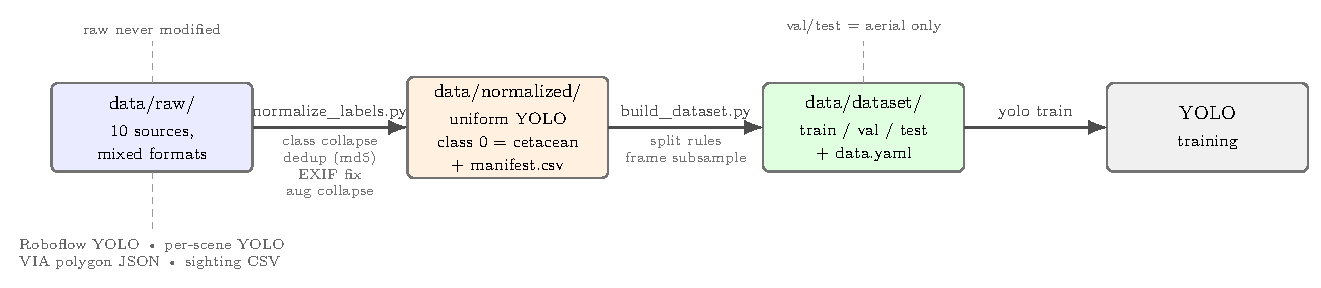
\includegraphics[width=\linewidth]{figures/data_pipeline.pdf}
\caption{Data-preparation pipeline. Ten raw sources in mixed formats
(Roboflow~YOLO, per-scene YOLO, VIA polygon JSON, sighting CSV) are converted
into a uniform single-class YOLO dataset (class collapse, MD5 deduplication,
EXIF-orientation correction, offline-augmentation collapse), then a dataset
builder materialises aerial-only validation/test splits. The raw data is never
modified.}
\label{fig:datapipe}
\end{figure}
\begin{itemize}[itemsep=2pt,topsep=2pt]
  \item \textbf{Content deduplication.} MD5 hashing removes byte-identical
  images that appear across sources, which eliminated cross-split leakage
  (e.g.\ Dryad images present in both train and test) and repeated UAV frames.
  \item \textbf{EXIF-orientation correction.} Many Dryad images carry EXIF
  orientation flags 3/6/8 while their VIA polygon coordinates are in the
  \emph{raw} pixel frame. The pipeline bakes the rotation into re-encoded JPEGs
  \emph{and} applies the matching coordinate transform (rot180, rot90CW,
  rot90CCW), verified per-orientation. Every other source was confirmed
  orientation-1.
  \item \textbf{Offline-augmentation collapse.} Roboflow exports bake in offline
  augmentation (original~+~flip~+~brightness under one stem). These were
  collapsed to one instance per original image, which byte-level dedup misses
  since flips change the bytes. Only training splits are affected; val/test are
  left intact.
\end{itemize}
\noindent After normalisation the dataset contains \textbf{$27{,}290$ images /
$55{,}163$ boxes / $640$ background (negative) frames}. A dataset builder
then materialises train/val/test splits with the
invariant that \emph{validation and test are aerial-only}, that the
\texttt{whale-bbox-layer} source is held out \emph{whole} as a precision test
(no leakage of that domain into training), and that UAV video scenes are
split-disjoint and subsampled at scene level to avoid near-duplicate frames
leaking across splits.

\subsection{Scale analysis: a bimodal, porpoise-weighted dataset}\label{sec:scale}
Analysing box sizes both sets the tiling strategy and previews the GSD-axis
argument. The apparent-size distribution is strongly \emph{bimodal}
(Fig.~\ref{fig:sizedist}): a porpoise / small-delphinid mode near $40$~px,
supplied overwhelmingly by \texttt{uav-porpoises} ($84\%$ of all boxes), and a
whale / large-dolphin mode three orders of magnitude larger (medians of
$1300$--$1700$~px for \texttt{whaleshape}, \texttt{cetacean-detector},
\texttt{dryad}). The global median box $\sqrt{\text{area}}$ is $\approx\!45$~px,
landing in the sparse valley \emph{between} the two modes --- a subtlety that
matters when tuning inference (Section~\ref{sec:inference}), since a single
magnification target set at the global median serves \emph{neither} mode well.
Because most sources contain large in-frame animals and fewer than a per~cent of
boxes fall below $\sim\!10$~px at $\imgsz$~px input, tiling is deferred to the
\emph{inference} stage rather than baked into training; the working SAHI tile is
set by the small end (porpoise/screening regime) at $640$~px, overlap $0.2$,
model input $\imgsz$~px.

\begin{figure}[H]
\centering
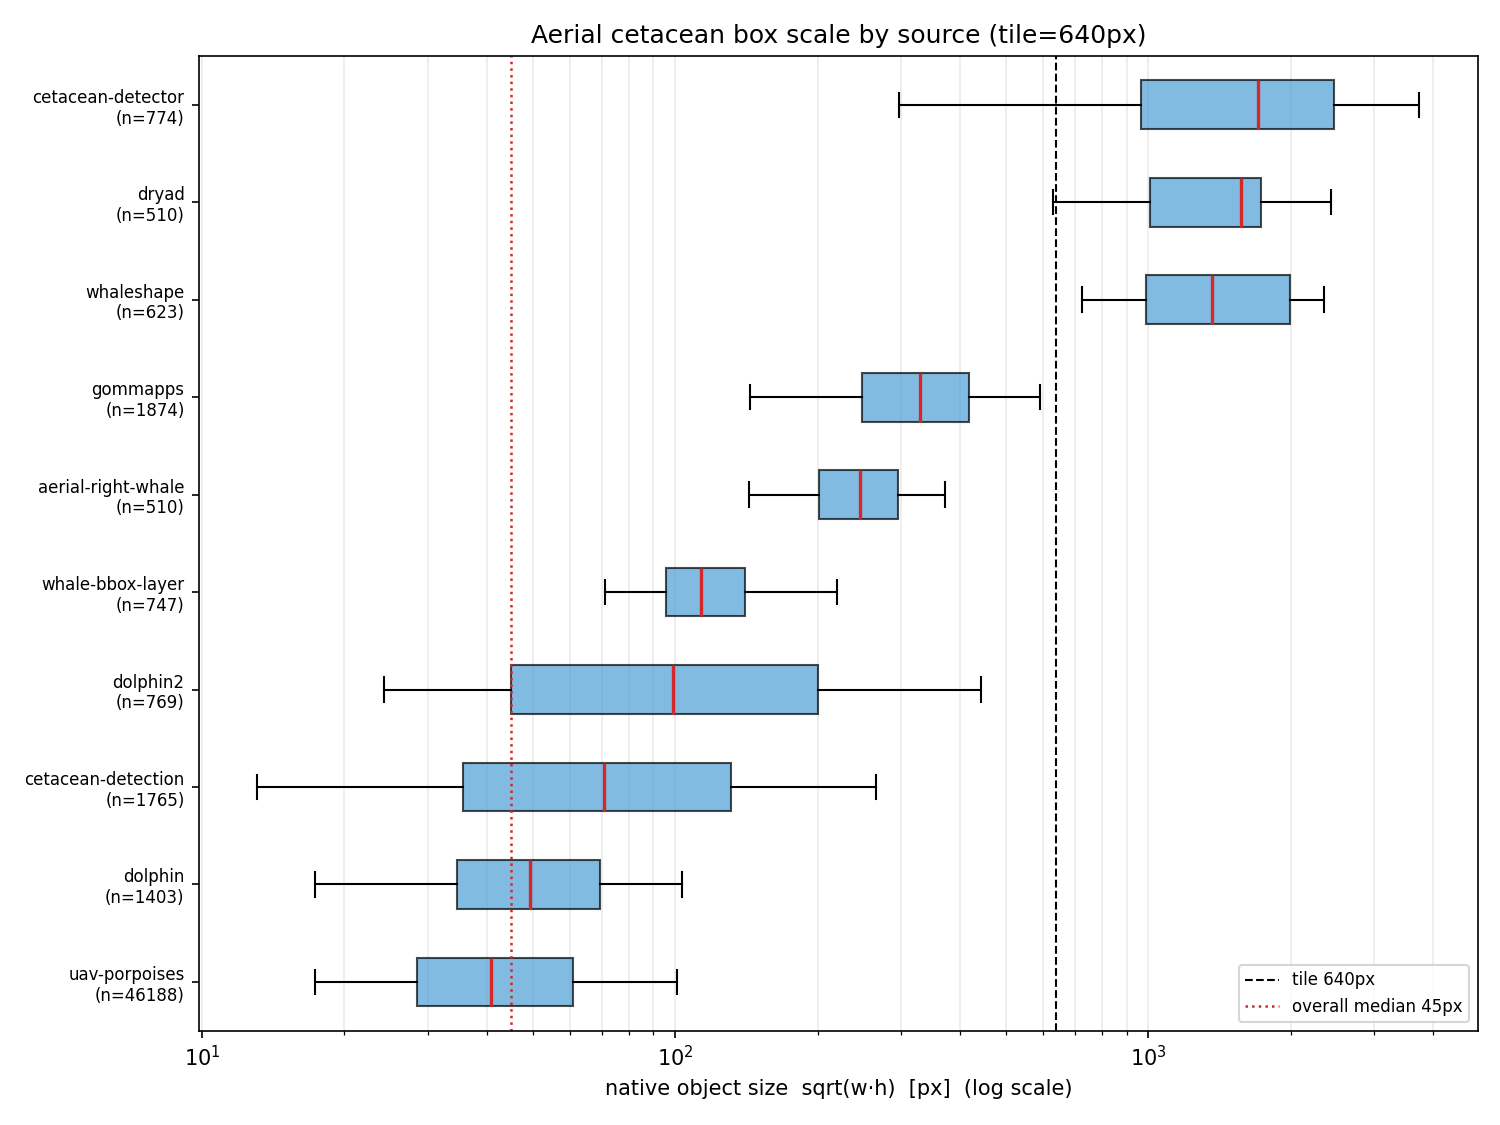
\includegraphics[width=0.92\linewidth]{figures/size_distribution.png}
\caption{Box-size distribution across sources (box $\sqrt{\text{area}}$, log
scale). The dataset is strongly \emph{bimodal}: a dominant porpoise /
small-delphinid mode near $40$~px (\texttt{uav-porpoises}, $84\%$ of boxes) and
a whale / large-dolphin mode three orders of magnitude larger. The global
median ($\approx\!45$~px) sits in the valley between the modes. This
three-order-of-magnitude spread within one single-class dataset is the physical
basis of the GSD axis: no single input scale can serve every altitude, which
motivates resolving scale at inference time (Section~\ref{sec:inference}).}
\label{fig:sizedist}
\end{figure}

\paragraph{A porpoise-weighted dataset is representative, not biased.}
This porpoise-heavy composition is not a sampling artefact: harbour porpoise and
small delphinids numerically dominate real North-East Atlantic shelf
populations, whereas large baleen whales are comparatively rare
\citep{hammond2013cetacean}. A dataset --- and a benchmark --- weighted toward
small targets is thus \emph{representative} of the operational species mix, and
the small-target recall floor it exposes is precisely the one that matters most
in deployment. Section~\ref{sec:screening} shows that this source is also
critical: removing it collapses the detector.

\subsection{Label Studio pseudo-labelling loop}\label{sec:labelstudio}
Labelled aerial cetacean data is scarce, but unlabelled aerial footage is easy
to obtain. We close this gap with a human-in-the-loop pseudo-labelling loop
(Fig.~\ref{fig:pipeline}) built on Label~Studio \citep{labelstudio}:
\begin{enumerate}[itemsep=2pt,topsep=2pt]
  \item \textbf{Predict.} The current best model is run over an unlabelled
  aerial pool (at low confidence so the human mostly corrects rather than draws)
  to produce pre-annotations.
  \item \textbf{Review.} A human accepts, corrects or rejects each box, keeping
  \emph{cetaceans only} --- an essential filter, because the source sighting
  logs also contain turtles, sharks and even ``whale shark'' (a fish) --- and
  applying a floor rule that skips ambiguous, faint low-contrast targets.
  \item \textbf{Merge.} Reviewed labels are folded back as a new normalised
  source and appended to the manifest.
  \item \textbf{Retrain.} The detector is retrained on the \emph{combined} set
  (never new-only, which causes forgetting), and a fixed held-out test set
  enables round-over-round comparison.
\end{enumerate}
The reviewed \texttt{gommapps} survey set ($420$ reviewed frames / $1{,}874$
boxes / $57$ empty) enters the dataset this way and contributes both positives
and, from its no-sighting frames, hard negatives (Section~\ref{sec:screening}).
The loop provides the scalable mechanism by which future AEROSUB survey flights
become training data.

\begin{figure}[H]
\centering
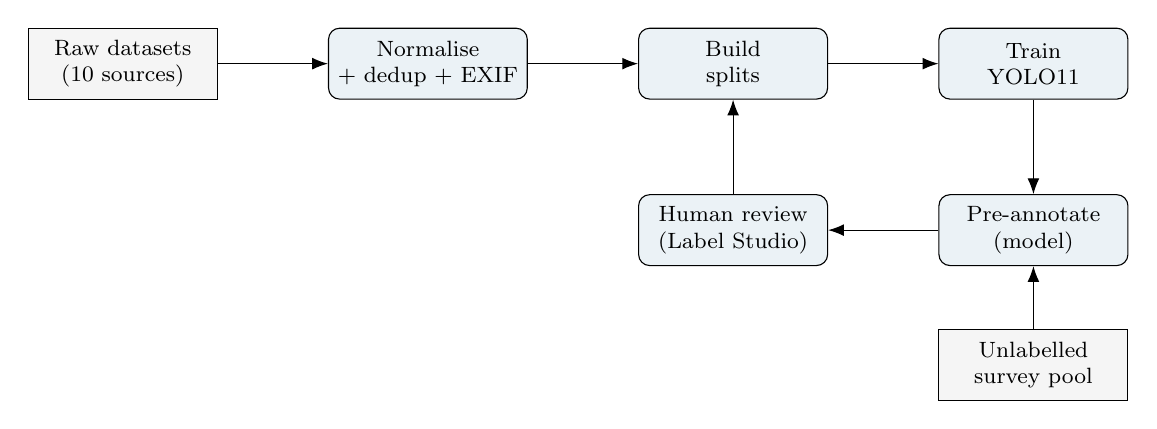
\begin{tikzpicture}[
  node distance=10mm and 14mm,
  box/.style={draw,rounded corners,align=center,minimum height=9mm,
              minimum width=24mm,font=\footnotesize,fill=slblue!8},
  data/.style={draw,align=center,minimum height=9mm,minimum width=24mm,
               font=\footnotesize,fill=black!4},
  arr/.style={-{Latex[length=2mm]}}]
\node[data] (raw) {Raw datasets\\(10 sources)};
\node[box,right=of raw] (norm) {Normalise\\+ dedup + EXIF};
\node[box,right=of norm] (build) {Build\\splits};
\node[box,right=of build] (train) {Train\\YOLO11};
\node[box,below=12mm of train]  (predict) {Pre-annotate\\(model)};
\node[box,below=12mm of build]  (review)  {Human review\\(Label Studio)};
\node[data,below=8mm of predict] (pool)    {Unlabelled\\survey pool};
\draw[arr] (raw)--(norm);
\draw[arr] (norm)--(build);
\draw[arr] (build)--(train);
\draw[arr] (train)--(predict);
\draw[arr] (pool)--(predict);
\draw[arr] (predict)--(review);
\draw[arr] (review)--(build);
\end{tikzpicture}
\caption{Data and pseudo-labelling pipeline. Curated datasets train the
detector; the detector pre-annotates unlabelled survey footage; a human
reviewer corrects the labels; corrected data re-enters the combined training
dataset.}
\label{fig:pipeline}
\end{figure}

% =====================================================================
\section{The Detector and the Screening Study}\label{sec:screening}
% =====================================================================
\subsection{Detector and training}
We use \textbf{YOLO11} \citep{khanam2024yolov11,ultralytics2023yolo}, a
single-class detector at input resolution $\imgsz$~px. Training uses the
Ultralytics framework (v8.4) on a single Quadro RTX~4000 (8\,GB): batch~$18$,
up to $100$ epochs with early stopping (patience~$20$), fixed seed $1337$. We
keep augmentation view-agnostic --- vertical flips and large rotations are
label-preserving only for nadir imagery and corrupt oblique frames, so the
global schedule uses horizontal flip, HSV, scale, translate and mosaic only. A
view-conditional strategy is left as future work. The baseline M1 converges
cleanly under this schedule: training and validation losses fall in step (no
over-fitting) and validation \map{} plateaus by epoch $\sim\!80$
(Fig.~\ref{fig:baselinecurves}).

\begin{figure}[ht]
\centering
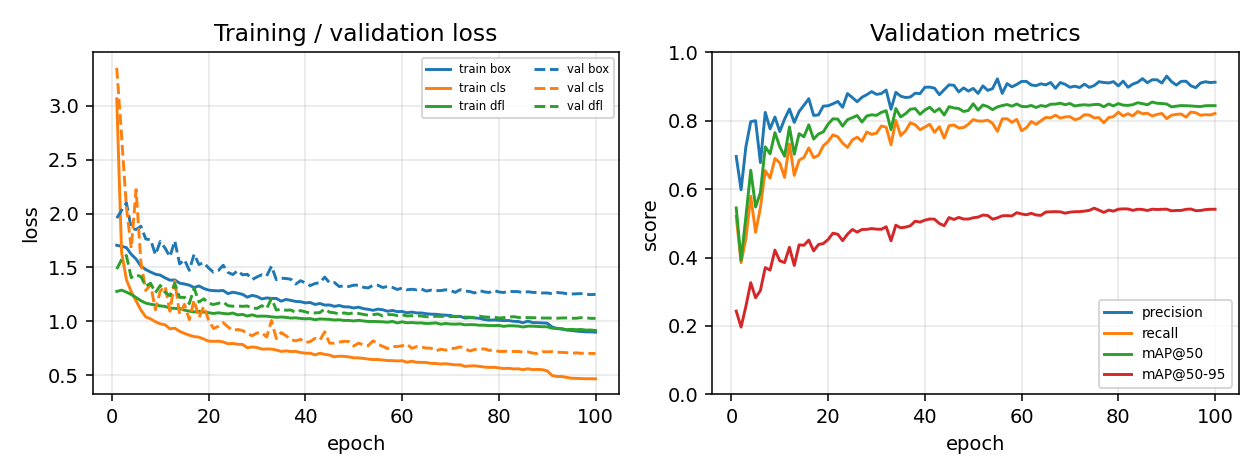
\includegraphics[width=\linewidth]{figures/baseline_curves.png}
\caption{Baseline detector (M1, YOLO11n) training. Left: training (solid) and
validation (dashed) box/cls/dfl losses fall together, indicating no over-fitting.
Right: validation precision, recall and \map{} rise and plateau
($\map50\approx0.84$, $\map50\text{-}95\approx0.54$ at epoch $100$).}
\label{fig:baselinecurves}
\end{figure}

\paragraph{Two operating points, two metrics.}
Following the GSD-axis argument, we evaluate the detector at both ends of the
axis on fixed, held-out data:
\begin{itemize}[itemsep=2pt,topsep=2pt]
  \item \textbf{High-GSD, exact detection.} A held-out \emph{source}
  (\texttt{whale-bbox-layer}, $106$ images / $153$ instances, never seen in
  training) measures precision and \map{} at $\text{IoU}\!\ge\!0.5$ under plain
  inference. An in-distribution aerial slice ($291$ images, porpoise-dominated)
  is reported alongside.
  \item \textbf{Low-GSD, screening.} An external HiDef Aerial Surveying digital
  aerial survey (denoted the \emph{HiDef} test set; $704$ frames / $838$ boxes /
  $12$ empty, fully held out, a \emph{different} survey domain;
  Fig.~\ref{fig:hidef}) measures recall against false positives
  per image (recall@$\fppi$, IoU~$\ge\!0.3$ one-to-one match) under SAHI tiling ---
  the screening/FROC metric.
\end{itemize}

\paragraph{A controlled six-way study.}
To find which choices move each operating point we change \emph{one} factor at a
time from a baseline \textbf{M1} (YOLO11n; aerial sources; porpoises in;
$10\%$ hard-negative dose), holding seed and schedule fixed (Table~\ref{tab:exp}).

\begin{table}[t]
\centering
\caption{The six controlled training configurations. Each changes one factor
from baseline \textbf{M1}. Dose = negatives as a fraction of the final training
set; \emph{Train img.}\ is the number of images in that config's training split.
All evaluated on the identical fixed test sets. Note how removing the porpoise
source (M4) shrinks the training set threefold --- a first sign of how
indispensable it is.}
\label{tab:exp}
\small
\setlength{\tabcolsep}{5pt}
\begin{tabular}{llrl}
\toprule
Variant & Backbone & Train img. & Change from M1 \\
\midrule
M1  & YOLO11n & 5{,}394 & baseline (aerial, porpoises in, $10\%$ neg) \\
M2  & YOLO11s & 5{,}394 & \emph{capacity} $\uparrow$ (same data as M1) \\
M3  & YOLO11n & 8{,}618 & $+$ four surface sources \\
M4  & YOLO11n & 1{,}506 & porpoise source \emph{removed} \\
M5  & YOLO11n & 4{,}855 & hard-negative dose $0\%$ \\
M6  & YOLO11n & 6{,}069 & hard-negative dose $20\%$ \\
\bottomrule
\end{tabular}
\end{table}

\subsection{High-GSD result: exact detection}
Table~\ref{tab:precision} reports the precision regime. On the held-out
\texttt{whale-bbox-layer} source the models cluster tightly
($\map50 \approx 0.50$--$0.54$), and \emph{capacity barely moves it}: the
YOLO11s variant M2 ($\map50\ 0.540$) is within a point of the YOLO11n
baseline M1 ($0.538$). Removing porpoises (M4) is the one large effect, and it is
strongly negative ($\map50\ 0.202$): even for large-whale precision, the
porpoise source is critical. Extra surface data (M3) slightly hurts, and
hard-negative dose trades a little precision for a little recall. The takeaway of
the high-GSD end is that, once the animal is resolved, this task is
capacity-insensitive and configuration-robust --- backbone capacity is not the
bottleneck.

\begin{table}[H]
\centering
\caption{High-GSD \textbf{exact-detection} regime, plain inference at $\imgsz$~px.
Held-out source = \texttt{whale-bbox-layer} ($106$ img / $153$ inst); aerial
slice = in-distribution ($291$ img, porpoise-dominated). Capacity (M2) barely
changes \map; removing porpoises (M4) collapses even large-animal precision.}
\label{tab:precision}
\small
\setlength{\tabcolsep}{5pt}
\begin{tabular}{llcccc}
\toprule
 & & \multicolumn{2}{c}{Held-out source} & \multicolumn{2}{c}{Aerial slice} \\
\cmidrule(lr){3-4}\cmidrule(lr){5-6}
Variant & Backbone & \map50 & \map50\text{-}95 & \map50 & \map50\text{-}95 \\
\midrule
M1  & 11n & 0.538 & 0.221 & 0.824 & 0.520 \\
M2  & 11s & \textbf{0.540} & \textbf{0.227} & \textbf{0.863} & \textbf{0.550} \\
M3  & 11n & 0.510 & 0.238 & 0.793 & 0.508 \\
M4  & 11n & 0.202 & 0.070 & 0.143 & 0.093 \\
M5  & 11n & 0.531 & 0.212 & 0.823 & 0.532 \\
M6  & 11n & 0.503 & 0.224 & 0.801 & 0.521 \\
\bottomrule
\end{tabular}
\end{table}

\subsection{Low-GSD result: wide-area screening}
\begin{figure}[ht]
\centering
\begin{subfigure}{\linewidth}
  \centering
  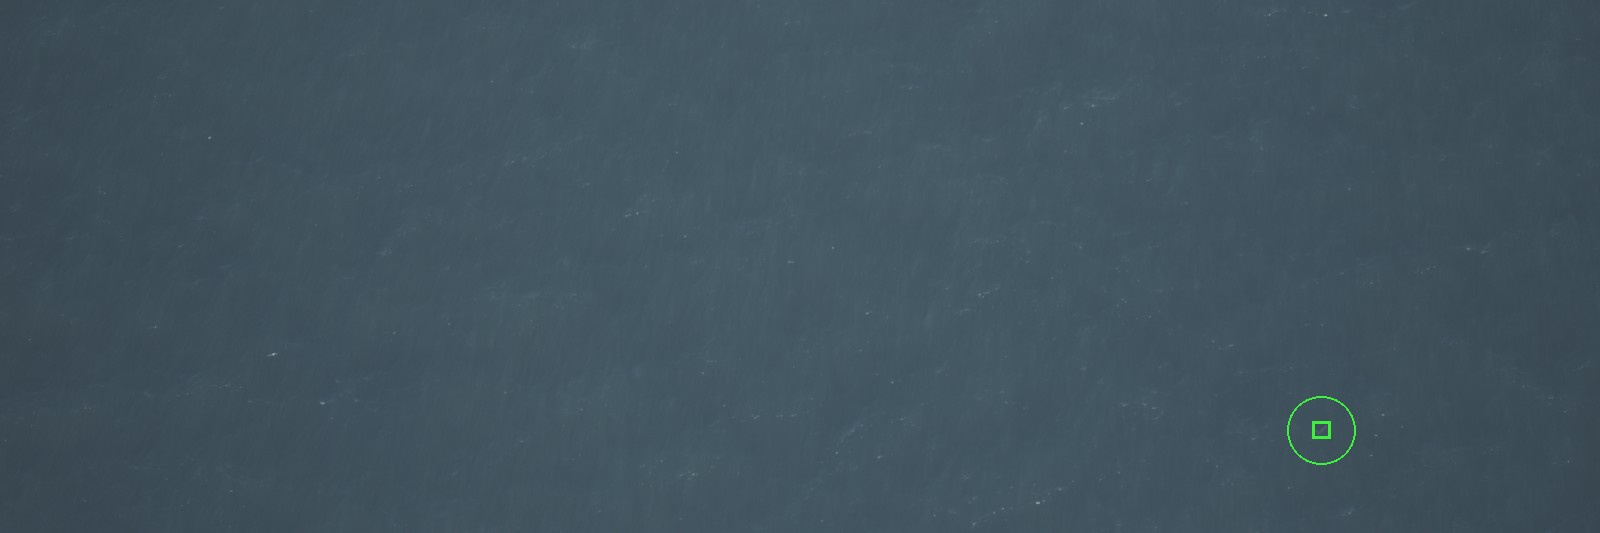
\includegraphics[width=\linewidth]{figures/hidef_frame.jpg}
  \caption{A HiDef survey frame (downscaled to fit the column): one confirmed
  harbour porpoise (green box, ringed for visibility) in an otherwise empty sea.}
\end{subfigure}

\vspace{5pt}
\begin{subfigure}{0.5\linewidth}
  \centering
  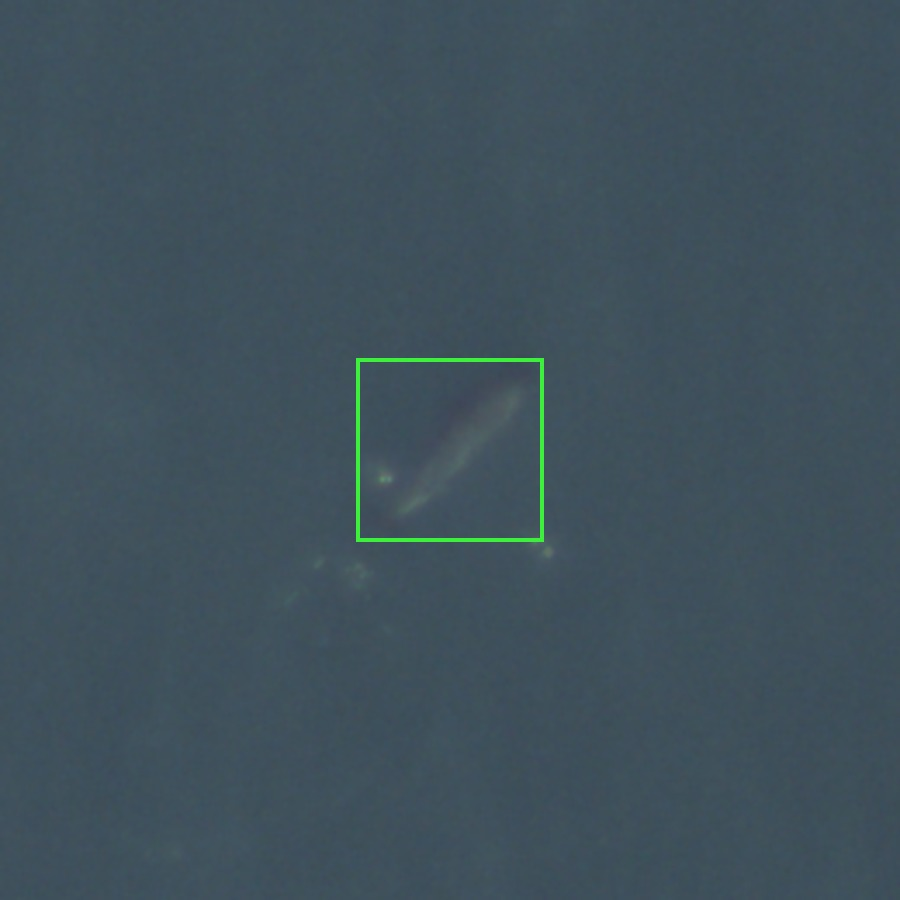
\includegraphics[width=\linewidth]{figures/hidef_zoom.jpg}
  \caption{Magnified crop of that porpoise: only $\approx\!50$~px across at the
  survey's native resolution --- a faint, low-contrast target.}
\end{subfigure}
\caption{The low-GSD \emph{screening} regime on the held-out HiDef Aerial
Surveying digital aerial survey. At this ground-sample distance a harbour
porpoise occupies only a few tens of pixels in a multi-megapixel frame, so exact
species identification from a single frame is impossible and the appropriate task is
high-recall triage: cueing a human expert to the frame (and tile) that contains
an animal.}
\label{fig:hidef}
\end{figure}

The screening regime shows the opposite pattern (Table~\ref{tab:froc},
Fig.~\ref{fig:froc}). Here \emph{capacity matters}: the YOLO11s variant M2
lifts recall at $1$ false positive per image from M1's $0.412$ to
\textbf{$0.535$} --- a $30\%$ relative gain --- and dominates at the tight
operating points ($0.240$ vs $0.063$ recall at $0.1\ \fppi$). The larger
backbone helps exactly where the target is a few low-contrast pixels and shape
must be inferred, which is the opposite of the common ``nano is enough for edge
detection'' assumption. Composition again dominates the rest:
\begin{itemize}[itemsep=2pt,topsep=2pt]
  \item \textbf{Porpoises are essential.} M4 (porpoises removed) is flat on the
  floor ($\le\!0.04$ recall at every budget): a detector that never learned that
  a faint, low-contrast target can be an animal cannot screen at low GSD.
  \item \textbf{Surface data hurts.} M3 ($+$surface) sits well below M1/M2;
  boat-deck and close-range imagery pulls the detector away from the nadir
  screening regime.
  \item \textbf{Hard negatives trade recall for precision.} In the
  recall-oriented screening regime \emph{fewer} negatives is better at loose
  budgets: M5 ($0\%$) reaches $0.635$ recall at $2\ \fppi$ versus M1's $0.573$
  and M6's $0.443$. Hard negatives buy precision at a cost in the recall we
  care about here.
\end{itemize}
We also find that the coarser SAHI tile ($1024$~px) is both more accurate for
the strong configurations \emph{and} $\approx\!28\%$ cheaper than $640$~px on
these frames, so it is the preferred screening operating point.

\begin{table}[t]
\centering
\caption{Low-GSD \textbf{screening} regime on the out-of-domain HiDef
survey ($704$ frames), SAHI tile $1024$~px. Box-level recall at a false-positive
budget (IoU~$\ge\!0.3$). Best per column in bold. Capacity (M2) and porpoise
inclusion govern the floor; M4 collapses.}
\label{tab:froc}
\small
\setlength{\tabcolsep}{6pt}
\begin{tabular}{lcccc}
\toprule
Variant & R@$0.1$ & R@$0.5$ & R@$1.0$ & R@$2.0$ \\
\midrule
M1  & 0.063 & 0.264 & 0.412 & 0.573 \\
M2  & \textbf{0.240} & \textbf{0.449} & \textbf{0.535} & 0.611 \\
M3  & 0.132 & 0.260 & 0.307 & 0.384 \\
M4  & 0.004 & 0.016 & 0.024 & 0.038 \\
M5  & 0.081 & 0.396 & 0.525 & \textbf{0.635} \\
M6  & 0.033 & 0.173 & 0.296 & 0.443 \\
\bottomrule
\end{tabular}
\end{table}

\begin{figure}[t]
\centering
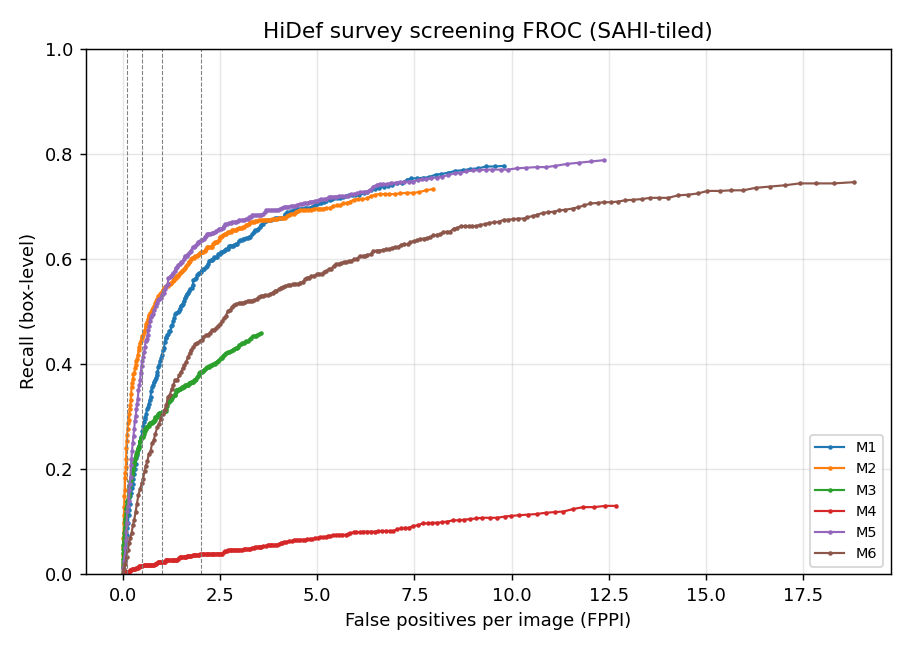
\includegraphics[width=0.82\linewidth]{figures/screening_froc.png}
\caption{Screening FROC on the out-of-domain HiDef survey (SAHI tile
$1024$~px): box-level recall vs.\ false positives per image. The larger-capacity
M2 (orange) and the negative-free M5 (purple) lead; the porpoise-free M4
(red) never leaves the floor. Dashed verticals mark the $0.1/0.5/1/2\ \fppi$
budgets of Table~\ref{tab:froc}. Recall plateaus near $0.6$--$0.65$ --- the
domain-gap ceiling of Section~\ref{sec:gap}.}
\label{fig:froc}
\end{figure}

\paragraph{What the detector catches --- and misses.}
Figure~\ref{fig:hidefgrid} makes the screening operating point concrete. At
$2\ \fppi$ the best-performing M2 recovers $513/838$ animals ($0.61$ recall):
despite being trained overwhelmingly on much larger whales, it reliably fires on
harbour porpoises only $\approx\!50$ apparent pixels across in a foreign survey
domain. Crucially the missed animals are \emph{not} smaller than the detected
ones --- both have a median box of $\approx\!50$~px (detected $49.4$~px, missed
$50.2$~px) --- so the low-GSD limit is set by \emph{contrast}, not raw size: the
misses are the faintest, lowest-contrast targets, animals under glare or against
dark, wake-broken water. Recovering three in five of these targets is a strong
screening result, and it is why more in-domain data
(Section~\ref{sec:labelstudio}), rather than a larger input, is the lever that
raises the floor.

\begin{figure}[ht]
\centering
\begin{subfigure}{0.49\linewidth}
  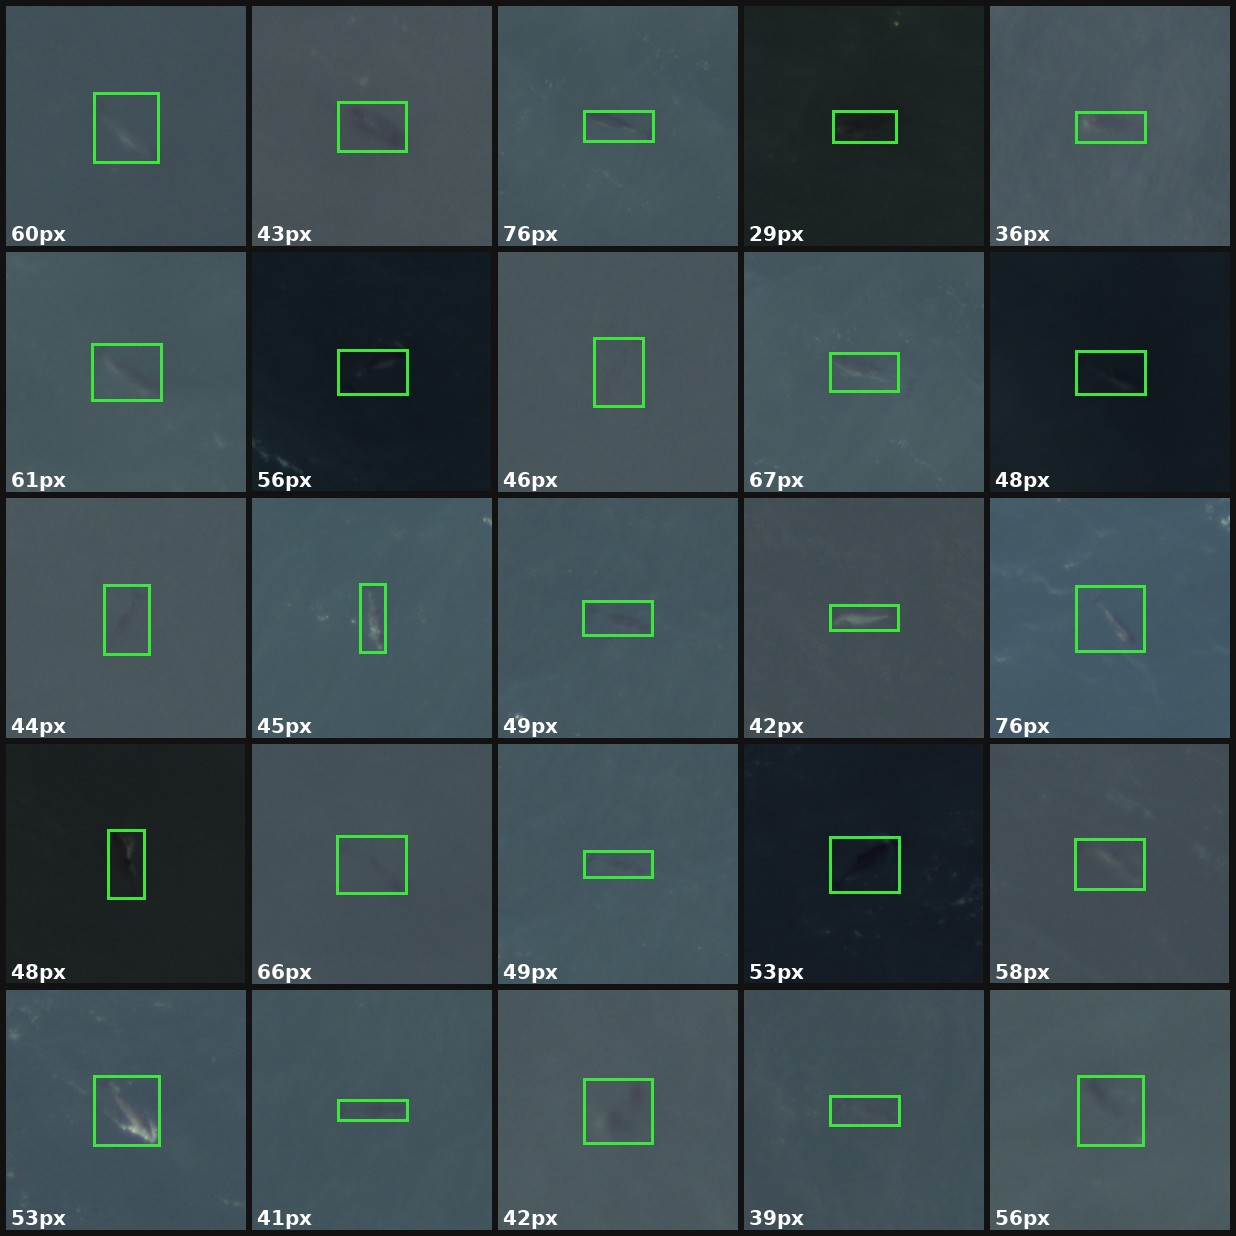
\includegraphics[width=\linewidth]{figures/hidef_detected.jpg}
  \caption{Detected ($25$ of $513$).}
\end{subfigure}\hfill
\begin{subfigure}{0.49\linewidth}
  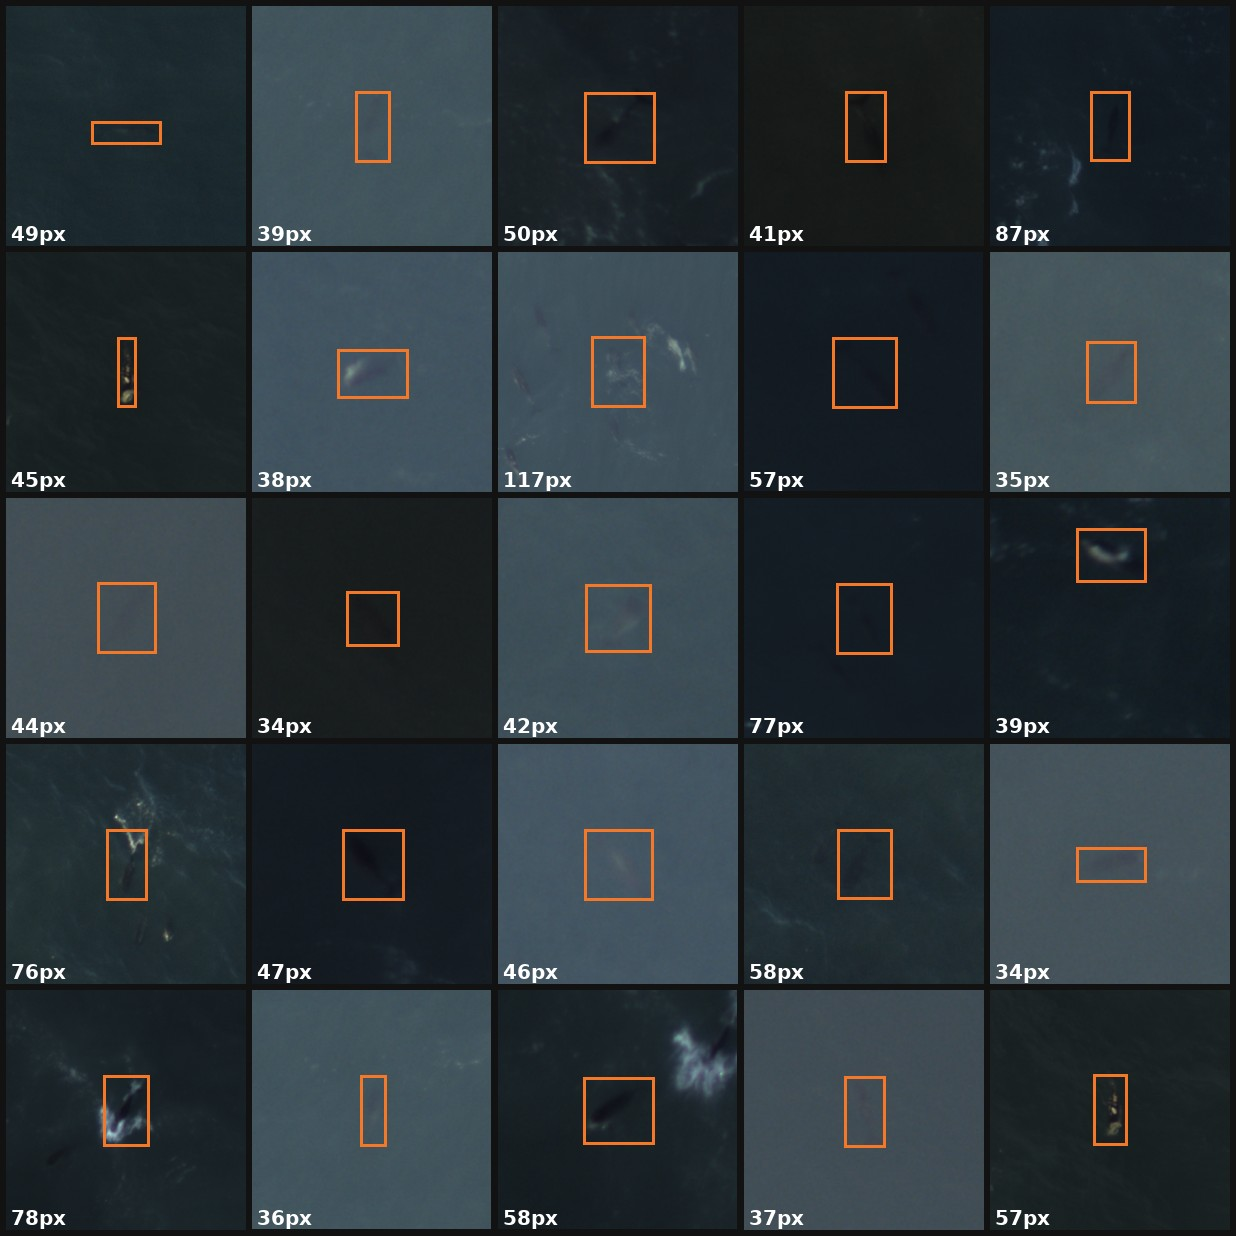
\includegraphics[width=\linewidth]{figures/hidef_missed.jpg}
  \caption{Missed ($25$ of $325$).}
\end{subfigure}
\caption{Best-performing M2 on the HiDef survey at the $2\ \fppi$ operating point
($0.61$ recall); each crop is centred on a ground-truth porpoise and labelled
with its native box size in pixels. (a) Detected and (b) missed animals are the
\emph{same} apparent size (median $\approx\!50$~px); the misses are simply the
lowest-contrast cases --- faint, low-contrast targets under glare or against dark,
wake-broken water --- not smaller animals.}
\label{fig:hidefgrid}
\end{figure}

\paragraph{Summary.}
The two operating points of one detector behave oppositely under the same
changes: high-GSD exact detection is capacity-insensitive and
configuration-robust, while low-GSD screening is capacity- and
composition-sensitive. The best-performing configuration overall is
\textbf{M2} (YOLO11s), which leads screening outright and matches the field at
exact detection; it is used for the scale-adaptive inference experiments below.

% =====================================================================
\section{Scale-Adaptive Inference}\label{sec:inference}
% =====================================================================
Sections~\ref{sec:scale} and~\ref{sec:screening} establish that the target's
\emph{apparent} size is the dominant variable. This section closes the loop with
inference geometry that holds apparent size roughly constant across the GSD axis.

\subsection{Why a fixed slice is rarely optimal}
Plain inference downscales the whole frame to $\imgsz$~px, so a target's apparent
size depends on field of view (altitude, lens, sensor), not on the sensor's
megapixel count. Extra megapixels help \emph{only through} tiling: on a
$151$-megapixel survey frame, plain inference detects nothing
(Section~\ref{sec:apem}); the animals are downscaled below the detection floor.
SAHI \citep{akyon2022sahi} runs the detector on overlapping tiles and merges the
results, but a \emph{fixed} tile size is rarely optimal: if tiles are too large
the animal is downscaled away; if too small, compute explodes and whitecaps and
glint are over-magnified into a large number of false positives. Two practical SAHI
findings recur throughout: the default confidence of $0.25$ is unreliable on water
and must be raised toward $0.5$, and SAHI's default non-maximum merging (NMM)
reconciles overlapping detections across tile seams more reliably than plain NMS.

\subsection{Adaptive SAHI: the scale solver}
\textbf{Adaptive SAHI} uses flight geometry to size tiles so a target is
re-magnified to a roughly constant apparent size at the model input, and
\emph{skips} tiling entirely when the animal is already large enough. Given
camera pixel pitch $p$, focal length $f$ and above-water altitude $h$, the
ground-sample distance and native target size are
\begin{align}
\mathrm{GSD} &= \frac{p\,h}{f}, &
\text{animal}_{\mathrm{px}} &= \frac{L_{\mathrm{target}}}{\mathrm{GSD}},
\end{align}
where $L_{\mathrm{target}}$ is the expected animal length. A survey frame of
long side $W$ is downscaled by $W/\imgsz$ before plain inference, so the detector
sees the animal at $a_{\text{plain}}=\text{animal}_{\mathrm{px}}\,\imgsz/W$
pixels. The solver uses one apparent-size target $a^\star$ (the trained
detection scale; here $a^\star\!\approx\!45$~px for a nominal
$L_{\mathrm{target}}\!=\!3$~m):
\begin{itemize}[itemsep=1pt,topsep=2pt]
  \item \emph{Skip rule.} If $a_{\text{plain}}\ge a^\star$ the animal is already
  detectable, so SAHI is skipped for a single plain pass.
  \item \emph{Slice rule.} Otherwise the crop size that renders the animal at
  $a^\star$ at model input $\imgsz$ is
  $\text{slice}=\text{animal}_{\mathrm{px}}\cdot \imgsz/a^\star$.
\end{itemize}
For the $151$-megapixel frame below (GSD~$2.41$~cm/px, so
$\text{animal}_{\mathrm{px}}\!\approx\!125$~px for a $3$~m animal) this yields
$\text{slice}\!\approx\!2834$~px --- large, few tiles, yet still magnifying the
pod far above the plain-inference floor.

\paragraph{A single length or a size range.}
Given one length the solver sizes a single slice for that scale. Given a size
\emph{range} $[L_{\min},L_{\max}]$ it instead sizes the crop so the
\emph{largest} expected animal still fits within one tile,
$\text{slice}=L_{\max}/(\mathrm{GSD}\cdot\phi)$ with fill fraction
$\phi\!\le\!1$. This \emph{range-aware} variant stops large whales being
fragmented across tile seams at low altitude, at the cost of more tiles; the
single-length policy is cheaper when the population is uniform.

\begin{figure}[t]
\centering
\resizebox{\linewidth}{!}{%
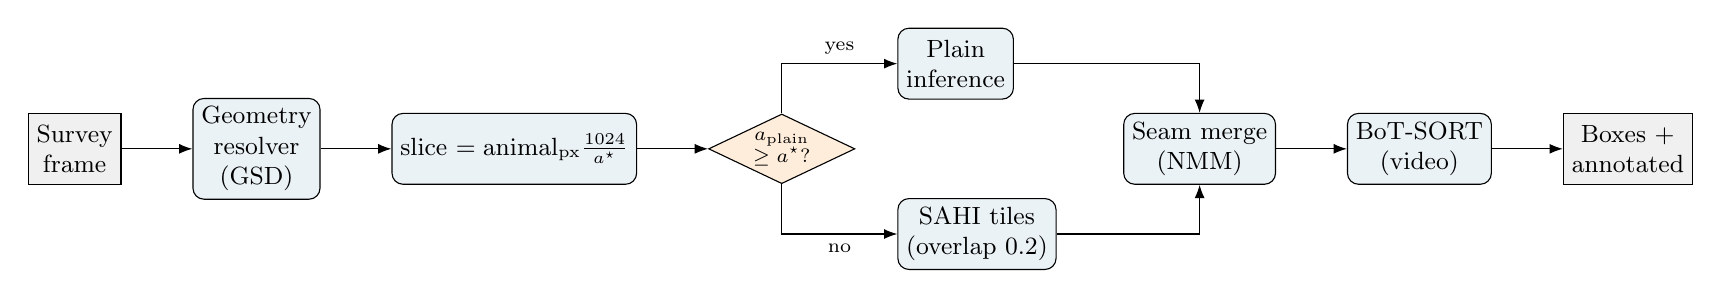
\begin{tikzpicture}[
  >=Latex, node distance=6mm and 9mm,
  box/.style={draw, rounded corners, align=center, minimum height=9mm,
              inner sep=3pt, font=\small, fill=slblue!8},
  io/.style ={draw, align=center, minimum height=9mm, inner sep=3pt,
              font=\small, fill=gray!12},
  dec/.style={draw, diamond, aspect=2.1, align=center, inner sep=1pt,
              font=\scriptsize, fill=orange!14}]
\node[io]  (frame) {Survey\\frame};
\node[box, right=of frame] (geo)  {Geometry\\resolver\\(GSD)};
\node[box, right=of geo]   (size) {slice $=\text{animal}_{\mathrm{px}}\frac{\imgsz}{a^\star}$};
\node[dec, right=of size]  (skip) {$a_{\text{plain}}$\\$\ge a^\star$?};
\node[box, above right=4mm and 10mm of skip] (plain) {Plain\\inference};
\node[box, below right=4mm and 10mm of skip] (sahi)  {SAHI tiles\\(overlap 0.2)};
\node[box, right=34mm of skip] (merge) {Seam merge\\(NMM)};
\node[box, right=of merge] (track) {BoT-SORT\\(video)};
\node[io,  right=of track] (out)   {Boxes +\\annotated};
\draw[->] (frame)--(geo);
\draw[->] (geo)--(size);
\draw[->] (size)--(skip);
\draw[->] (skip.north) |- (plain.west) node[pos=0.75, above, font=\scriptsize] {yes};
\draw[->] (skip.south) |- (sahi.west)  node[pos=0.75, below, font=\scriptsize] {no};
\draw[->] (plain.east) -| (merge.north);
\draw[->] (sahi.east)  -| (merge.south);
\draw[->] (merge)--(track);
\draw[->] (track)--(out);
\end{tikzpicture}}
\caption{Adaptive SAHI inference pipeline. Flight geometry sets the crop size;
frames whose animals are already detectable at plain resolution skip tiling
entirely, and video streams add BoT-SORT tracking after box merging.}
\label{fig:adaptivepipeline}
\end{figure}

\subsection{Scale-anchor cascade}
The solver needs one scale anchor, resolved by a fall-back cascade
(Fig.~\ref{fig:adaptivetree}) ordered from most to least reliable so the system
is autonomous whenever possible: (1) an explicit operator override; (2) a
user-/survey-supplied GSD or drone telemetry (DJI XMP \texttt{RelativeAltitude},
or EXIF altitude); (3) a per-flight camera model (pixel pitch, focal length)
plus altitude, giving GSD from the equation above; (4) with no geometry, a blind
sweep of $512/1024/2048$ keeping the most self-consistent result. All four tiers
are implemented and used below; a fifth self-calibration tier --- probing a
sparse subset and back-solving GSD from the first confident detection --- is
left as future work.

\begin{figure}[ht]
\centering
\resizebox{0.48\linewidth}{!}{%
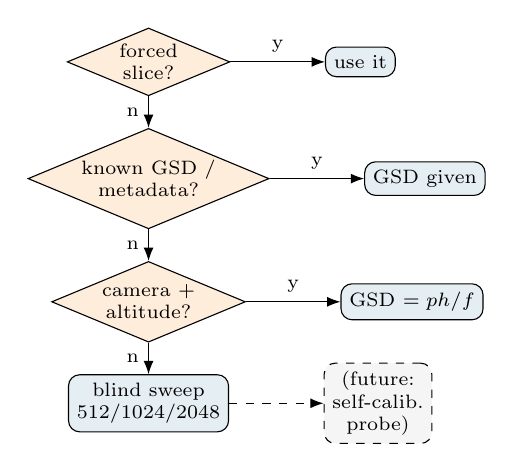
\begin{tikzpicture}[
  >=Latex, node distance=4mm and 12mm,
  q/.style={draw, diamond, aspect=2.4, align=center, font=\scriptsize,
            fill=orange!14, inner sep=1pt},
  a/.style={draw, rounded corners, align=center, font=\scriptsize,
            fill=slblue!10, inner sep=3pt},
  f/.style={draw, dashed, rounded corners, align=center, font=\scriptsize,
            fill=gray!8, inner sep=3pt}]
\node[q] (force) {forced\\slice?};
\node[a, right=of force] (fa) {use it};
\node[q, below=of force] (gsd)  {known GSD /\\metadata?};
\node[a, right=of gsd]   (ga) {GSD given};
\node[q, below=of gsd]   (cam)  {camera +\\altitude?};
\node[a, right=of cam]   (ca) {GSD $=ph/f$};
\node[a, below=of cam]   (blind) {blind sweep\\512/1024/2048};
\node[f, right=of blind] (self)  {(future:\\self-calib.\\probe)};
\draw[->] (force)--node[above,font=\scriptsize]{y}(fa);
\draw[->] (force)--node[left,font=\scriptsize]{n}(gsd);
\draw[->] (gsd)--node[above,font=\scriptsize]{y}(ga);
\draw[->] (gsd)--node[left,font=\scriptsize]{n}(cam);
\draw[->] (cam)--node[above,font=\scriptsize]{y}(ca);
\draw[->] (cam)--node[left,font=\scriptsize]{n}(blind);
\draw[->,dashed] (blind)--(self);
\end{tikzpicture}}
\caption{Scale-anchor cascade. Each answered branch resolves GSD (hence the crop
size); the self-calibration probe (dashed) is left for future work.}
\label{fig:adaptivetree}
\end{figure}

\subsection{Controlled altitude sweep}\label{sec:sweep}
Evaluating altitude behaviour needs matched frames of the \emph{same} animals at
many altitudes with exact ground truth --- data that does not exist for wild
cetaceans. We therefore build a \emph{semi-synthetic altitude sweep}: $18$ real,
model-verified animal cut-outs (lengths $1.7$--$18.2$~m, a realistic
porpoise-weighted mix) are feathered onto a real hard-negative ocean canvas
($8192\times5460$, stitched whitecap/glint tiles) and geometrically resampled
--- downscale only --- to the exact size each animal subtends at seven altitudes
($60$--$320$~m) under DJI~Zenmuse~P1 geometry ($p=4.39\,\mu$m, $f=35$~mm), so the
\emph{same} animals shrink with altitude on an unchanged sea texture
(Fig.~\ref{fig:sweepdata}). This
isolates the pure GSD variable while keeping textures photorealistic. For each frame
we compare plain inference, fixed-$640/1024$ SAHI, the single-length adaptive
policy and the range-aware variant, scoring recall, tile count and latency at
IoU~$\ge\!0.3$. Adaptive SAHI is an inference-time wrapper independent of the
trained weights: we drive it with the best-performing M2 here, and additionally run
baseline M1 on the real APEM frame (Table~\ref{tab:apem}) to confirm the
geometry-matched behaviour is not specific to one model (Table~\ref{tab:sweep},
Fig.~\ref{fig:sweep}).

\begin{figure}[ht]
\centering
\begin{subfigure}{\linewidth}
  \centering
  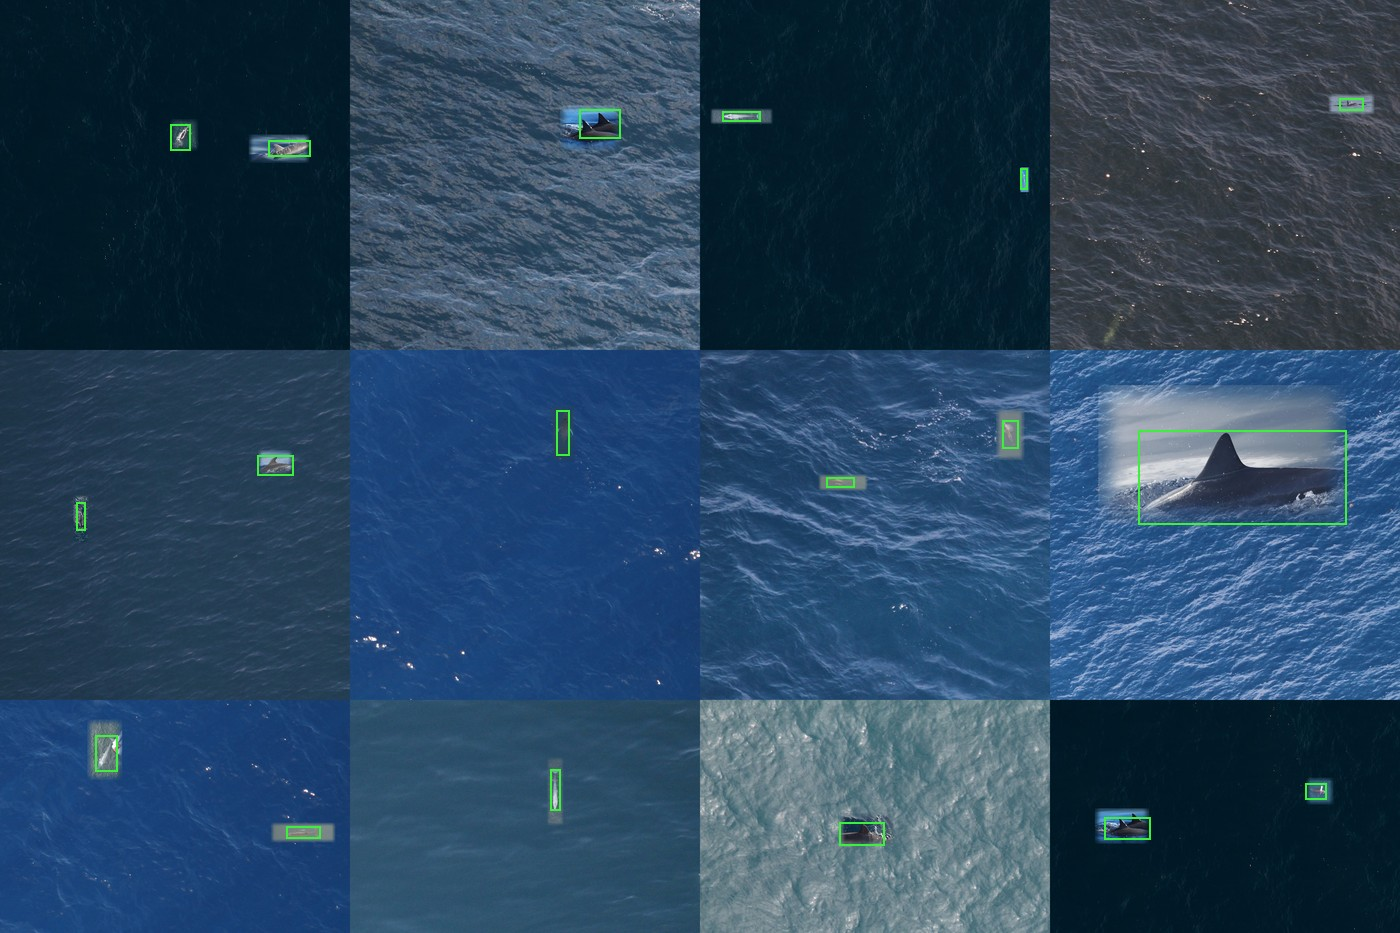
\includegraphics[width=0.86\linewidth]{figures/sweep_frame.jpg}
  \caption{One synthetic frame ($120$~m): $18$ model-verified cut-outs (green)
  feathered onto a real whitecap/glint canvas.}
\end{subfigure}

\vspace{4pt}
\begin{subfigure}{\linewidth}
  \centering
  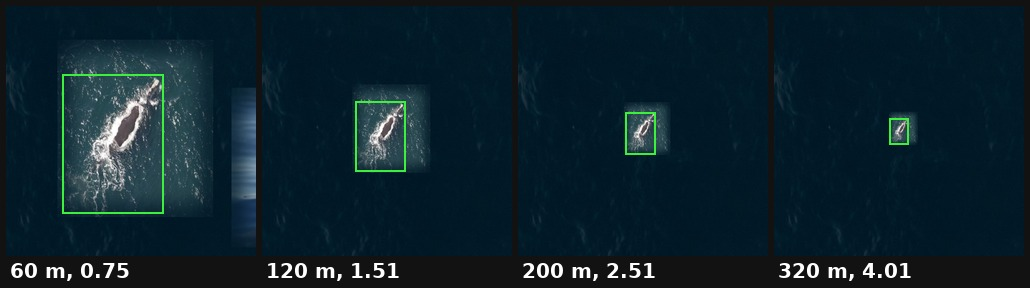
\includegraphics[width=0.86\linewidth]{figures/sweep_altitude_strip.jpg}
  \caption{The \emph{same} animal at four altitudes (label: altitude, GSD in
  cm/px): only the apparent size changes.}
\end{subfigure}
\caption{Semi-synthetic altitude sweep. Real animal cut-outs are composited onto
a real hard-negative ocean canvas and downscaled to the size each subtends at a
given altitude, isolating ground-sample distance from every other variable.}
\label{fig:sweepdata}
\end{figure}

\begin{table}[t]
\centering
\caption{Altitude sweep, best-performing M2: recall by altitude and tiles/frame per
method. Adaptive spends tiles only as geometry demands and \emph{approaches}
fixed-slice recall at a fraction of the cost, though fixed-$640$ keeps a recall
edge; \emph{range-aware} closes most of the gap at high altitude. At $60$~m the
adaptive skip rule (reasoning about a nominal $3$~m animal) reverts to plain and
loses the smaller animals --- a real, tunable limit (see text).}
\label{tab:sweep}
\small
\setlength{\tabcolsep}{5pt}
\begin{tabular}{lccccc}
\toprule
Alt.\ (GSD) & Plain & Fix-640 & Fix-1024 & Adaptive & Range-ad. \\
 & (1) & (176) & (70) & (1--24) & (1--280) \\
\midrule
60\,m (0.75) & 0.18 & \textbf{0.88} & 0.71 & 0.18 & 0.18 \\
120\,m (1.51) & 0.11 & 0.50 & 0.50 & 0.22 & 0.39 \\
200\,m (2.51) & 0.17 & 0.39 & 0.44 & 0.22 & \textbf{0.44} \\
320\,m (4.01) & 0.06 & 0.22 & 0.17 & 0.11 & 0.11 \\
\bottomrule
\end{tabular}
\end{table}

\begin{figure}[t]
\centering
\begin{subfigure}{0.49\linewidth}
  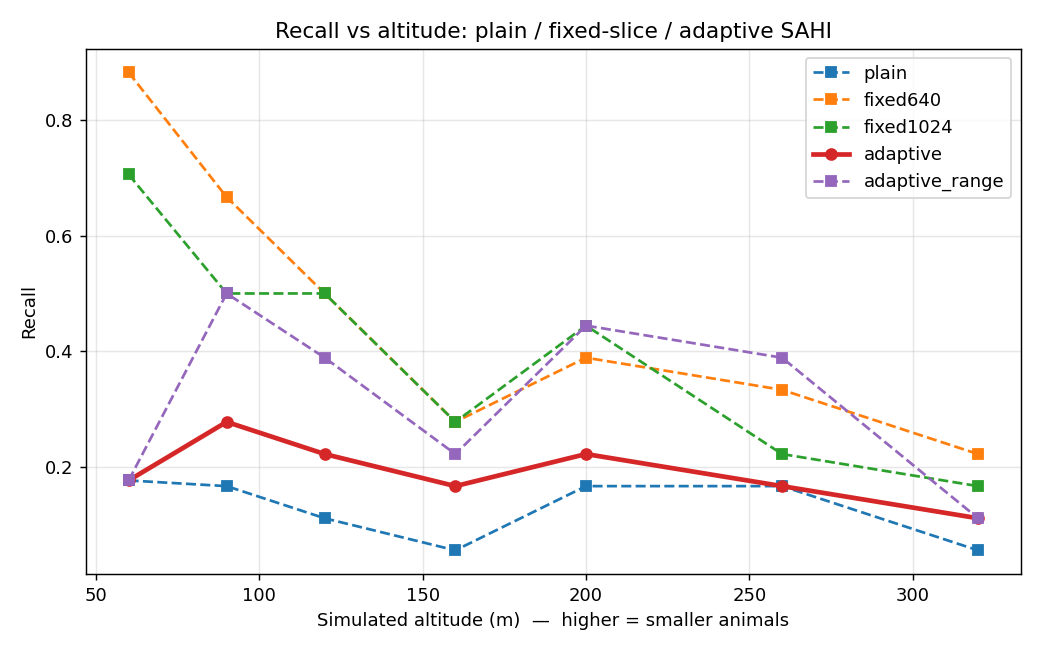
\includegraphics[width=\linewidth]{figures/sweep_recall.png}
  \caption{Recall vs.\ altitude}
\end{subfigure}\hfill
\begin{subfigure}{0.49\linewidth}
  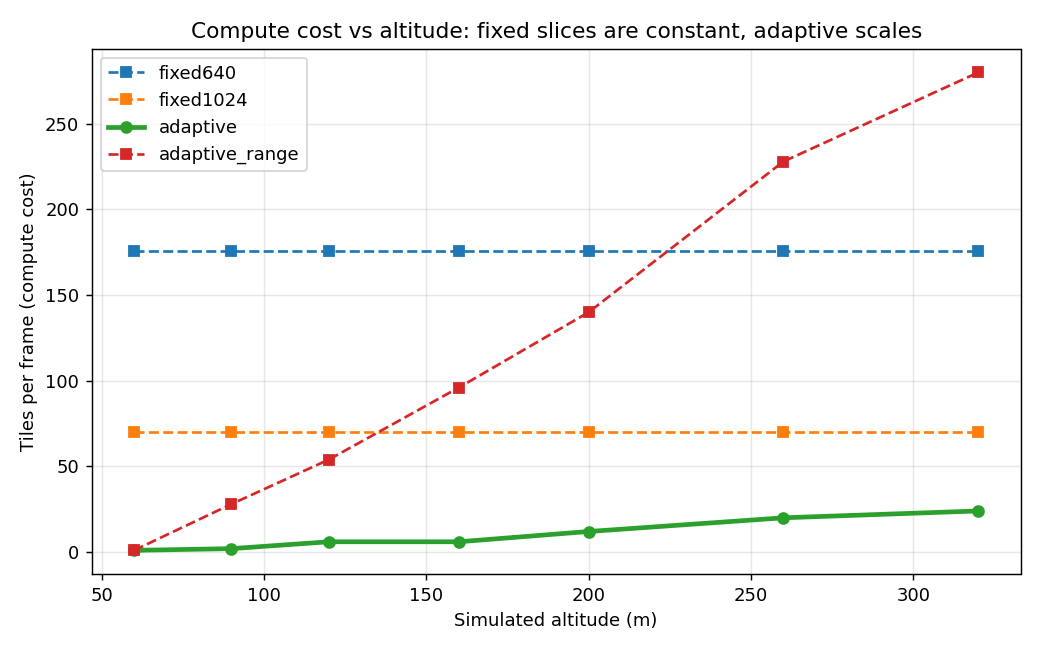
\includegraphics[width=\linewidth]{figures/sweep_tiles.png}
  \caption{Tiles/frame vs.\ altitude}
\end{subfigure}
\caption{Altitude sweep (best-performing M2). Adaptive approaches fixed-slice
recall at far fewer tiles (left; it does not exceed fixed slicing on recall)
while spending tiles only as altitude demands (right),
where fixed slicing pays a flat cost throughout. Above $\sim\!300$~m recall falls
for \emph{all} methods: once native detail is lost, no crop can restore it.}
\label{fig:sweep}
\end{figure}

\paragraph{A real limit at low altitude.}
At $60$~m the adaptive skip rule fires: a nominal $3$~m animal already subtends
$\approx\!50$~apparent pixels after the plain downscale, so the policy reverts to
a single plain pass and loses the sub-$3$~m animals that fixed-$640$ still
recovers ($0.18$ vs $0.88$). This is not a fundamental failure but a tuning
choice: setting $L_{\mathrm{target}}$ (or the skip threshold) to the
\emph{smallest} expected animal restores fine tiling at low altitude, at the cost
of more tiles. The default is deliberately conservative about compute; the point
of the sweep is that adaptive \emph{approaches} fixed recall at mid/high altitude
for far fewer tiles --- its advantage here is compute, not accuracy --- and that
the residual high-altitude decay is a scale-recovery limit shared by every
method, not a scheduling one.

\subsection{Real high-GSD anchor: a $151$-megapixel survey frame}\label{sec:apem}
We anchor the high-GSD, exact-detection end of the axis on a real survey frame
the detector has never seen: a $151$-megapixel APEM digital-aerial-survey frame
(Phase~One iXM-RS150F, $14204\times10652$~px) of three bottlenose dolphins, with
a recorded EXIF altitude of $448.5$~m giving GSD~$=2.41$~cm/px --- real geometry,
not an assumption. We report a single APEM frame because the provider's survey
imagery is proprietary and we were unable to obtain their dataset; this
publicly available frame is included as a representative high-GSD sample and to
show the wide variation in GSD and image quality \emph{between} survey vendors
--- contrast the coarse, low-contrast HiDef screening frames of
Fig.~\ref{fig:hidef} with this APEM stills frame, in which each dolphin is
cleanly resolved. Running the best-performing M2 at the slice its geometry anchor
dictates (Table~\ref{tab:apem}, Fig.~\ref{fig:apem}):
\begin{itemize}[itemsep=2pt,topsep=2pt]
  \item \textbf{Plain @$\imgsz$: 0/3.} After the $\sim\!14\times$ whole-frame
  downscale each dolphin is a handful of pixels; the detector finds nothing,
  even though the animals are clearly resolvable in the raw frame. Megapixels
  help only through tiling.
  \item \textbf{Fixed-$640$: 2/3 with $8$ false positives, $588$ tiles.} Fine
  tiles over-magnify whitecaps into porpoise-shaped false targets (the baseline M1
  produces $83$ false positives here), and the very finest pass still misses the
  faintest dolphin.
  \item \textbf{Adaptive (slice $2834$): 3/3 with $0$ false positives,
  $35$~tiles, $\approx\!9$~s.} Sizing the crop to the EXIF GSD recovers all
  three dolphins with no whitecap false alarms, at $17\times$ fewer
  tiles than fixed-$640$ and the fastest wall-clock of any method.
\end{itemize}
This is the key result of the high-GSD end: geometry-matched tiling turns an
apparently empty $151$-megapixel frame into a clean, complete detection, and
does so more cheaply than brute-force fine tiling because it magnifies the water
just enough to expose the animals and no further.

\begin{table}[t]
\centering
\caption{Real $151$-megapixel APEM frame (three bottlenose dolphins,
GSD~$2.41$~cm/px from EXIF). Recall (TP/FP) and tiles per method, IoU~$\ge\!0.3$.
Plain sees nothing; adaptive is complete, clean and cheapest. Baseline M1 shown
for the whitecap-false-positive contrast at fine tiles.}
\label{tab:apem}
\small
\setlength{\tabcolsep}{6pt}
\begin{tabular}{lccc}
\toprule
Method & Tiles & M2: R (TP/FP) & M1: R (TP/FP) \\
\midrule
Plain      & 1   & 0.00 (0/0) & 0.00 (0/0) \\
Fixed-640  & 588 & 0.67 (2/8) & 0.67 (2/83) \\
Fixed-1024 & 234 & 0.67 (2/0) & 1.00 (3/23) \\
\textbf{Adaptive} & \textbf{35} & \textbf{1.00 (3/0)} & 1.00 (3/1) \\
\bottomrule
\end{tabular}
\end{table}

\begin{figure}[ht]
\centering
\begin{subfigure}{0.57\linewidth}
  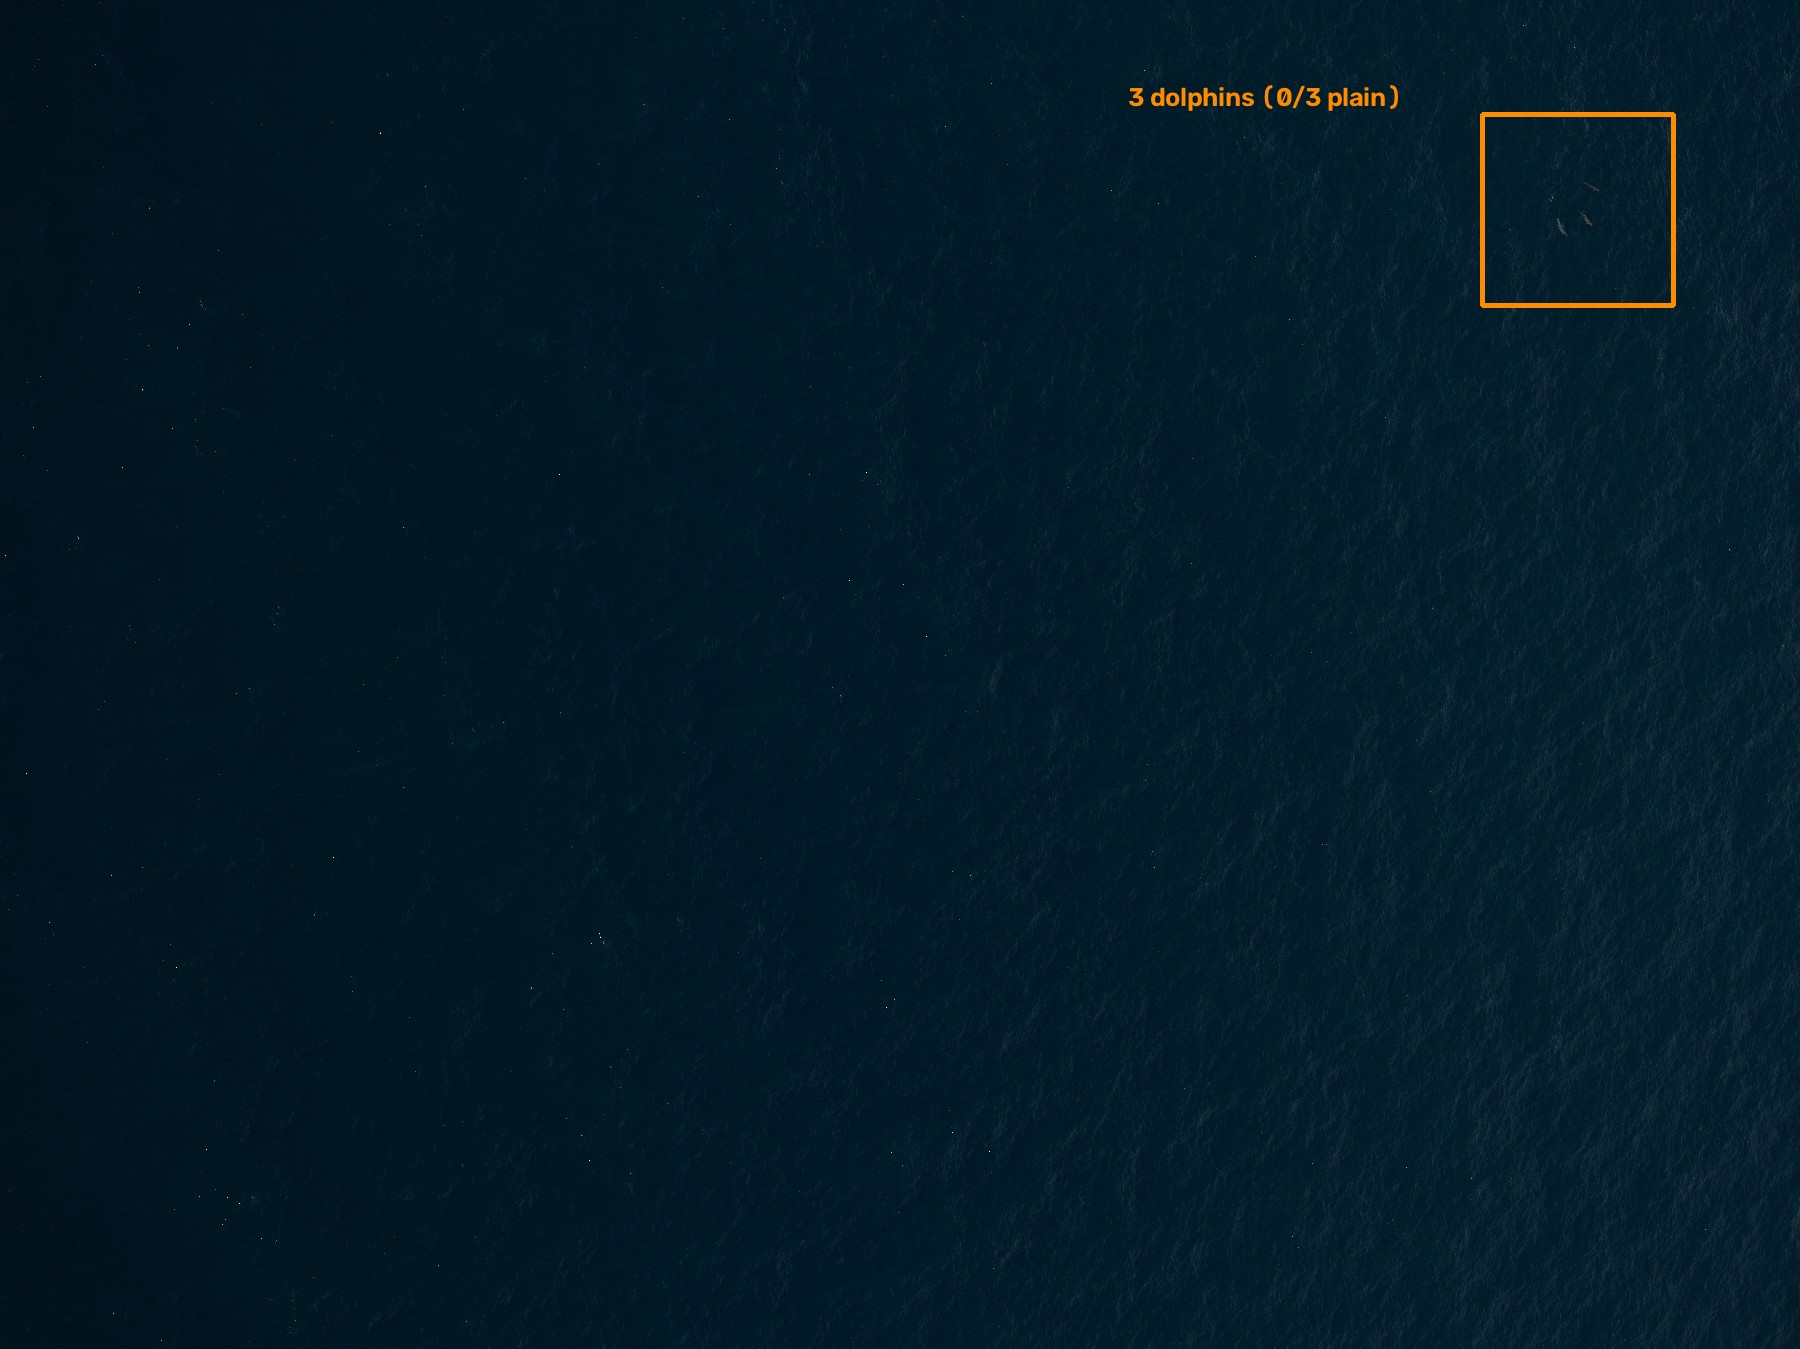
\includegraphics[width=\linewidth]{figures/apem_full_marked.jpg}
  \caption{Whole $151$~MP frame, plain @$\imgsz$: $0/3$. The pod is the marked
  cluster near the top-right; everything else is open water.}
\end{subfigure}\hfill
\begin{subfigure}{0.40\linewidth}
  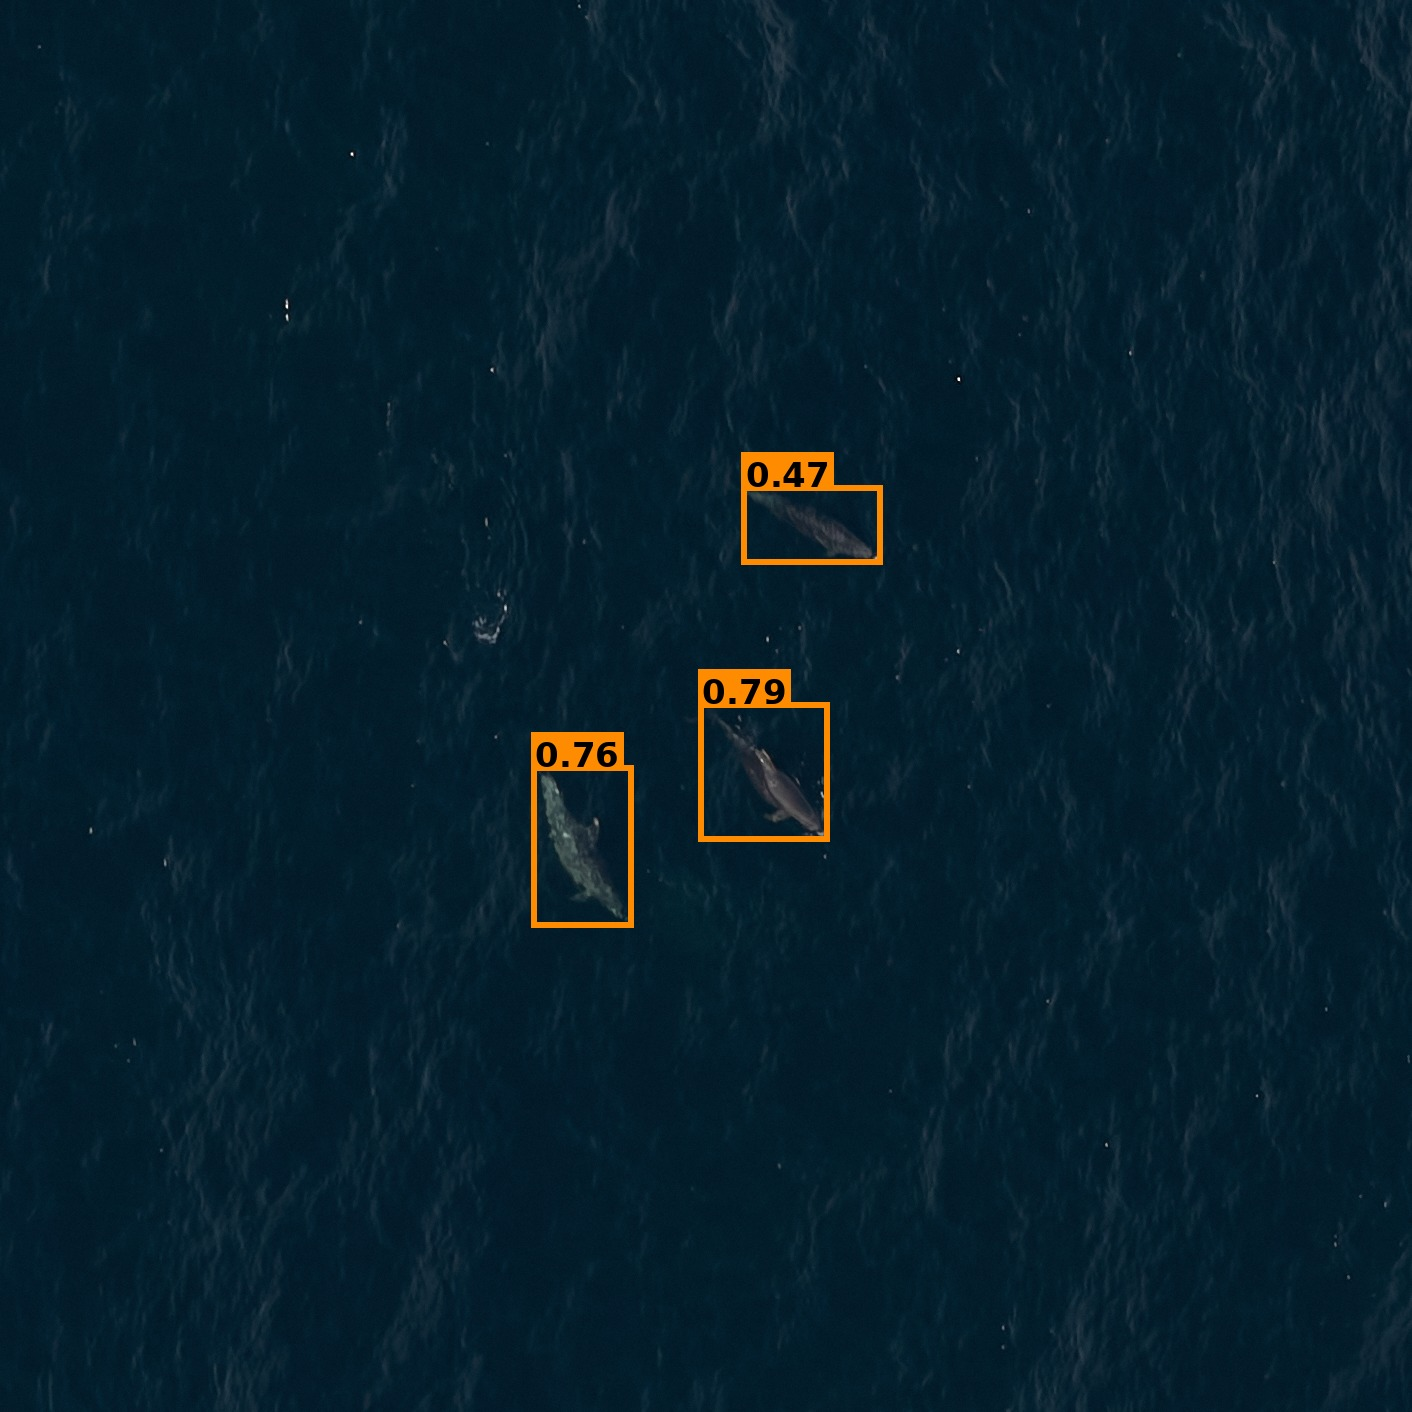
\includegraphics[width=\linewidth]{figures/apem_slice_boxes.jpg}
  \caption{Adaptive slice ($2834$~px) over the pod: $3/3$, $0$ FP (orange boxes,
  with confidences).}
\end{subfigure}
\caption{Real $151$-megapixel APEM survey frame (Phase~One iXM-RS150F,
GSD~$2.41$~cm/px). Whole-frame plain inference (left) detects none of the three
dolphins after the $\sim\!14\times$ downscale, even though the pod (marked) is
clearly resolvable in the raw pixels; adaptive SAHI, sized to the EXIF geometry,
recovers all three in a single geometry-matched crop (right) with zero whitecap
false positives, at $35$ tiles.}
\label{fig:apem}
\end{figure}

% =====================================================================
\section{The GSD Axis and the Domain Gap}\label{sec:gap}
% =====================================================================
The two real anchors bound the same detector at opposite ends of the GSD axis:
adaptive inference recovers the full three-dolphin pod on the single high-GSD
APEM frame, while at low GSD on the out-of-domain HiDef survey the best
configuration plateaus near $0.6$ recall at $2\ \fppi$ (Fig.~\ref{fig:froc}).
Both are direct measurements of one model; the gap between them is the subject
of this section.

\paragraph{Separating GSD from domain shift.}
The low-GSD screening ceiling confounds two effects: the animals are small
\emph{and} the survey is a different domain (different sensor, look and sea
state) from the training sources. Our two other experiments deliberately
separate them. The semi-synthetic sweep (Section~\ref{sec:sweep}) varies
\emph{only} GSD on in-domain textures and shows that recall degradation with
altitude is a scale-recovery effect shared by all inference methods --- pure GSD.
The HiDef survey adds domain shift on top of low GSD, and the extra
drop (recall capped near $0.6$ even with tiling) is the \emph{domain-gap}
component. In other words, we train on one set of aerial domains and deploy on a
different one, and the HiDef survey is a stress test of that transfer,
not a like-for-like test.

\paragraph{Why this is the right way to report it.}
Reporting a single aggregate number would hide this structure. Framed along the
GSD axis, the results are actionable: at high GSD the system is
deployment-ready and its remaining work is engineering (on-board packaging,
Section~\ref{sec:ros}); at
low GSD it is a \emph{screening aid} with a stated recall of $\approx\!0.5$--$0.6$
at a low false-alarm budget --- enough to cut an expert's review queue by
roughly half, but not a replacement for the observer. The levers that raise the
low-GSD floor are now known and quantified: more capacity (M2), the porpoise
source (M4), a low hard-negative dose (M5), and, above all, more in-domain
labelled data via the pseudo-labelling loop (Section~\ref{sec:labelstudio}).

\paragraph{Limitations.} Three caveats bound these claims. (i) The high-GSD
accuracy result is a \emph{single-frame demonstration}: the $3/3$, $0$-FP
outcome rests on one real APEM frame (three dolphins) plus a semi-synthetic
sweep, because provider survey imagery is proprietary
(Section~\ref{sec:apem}); broader validation across many real high-GSD frames
and surveys remains future work. (ii) On the synthetic sweep, adaptive SAHI's
demonstrated benefit is tile efficiency at \emph{comparable} recall, not higher
recall than fixed slicing (Table~\ref{tab:sweep}); the accuracy advantage is
shown only on the single APEM frame. (iii) Every configuration is a single
training run at one seed ($1337$) with no confidence intervals, so single-run
deltas (e.g.\ the $\approx\!30\%$ M2 screening gain) are indicative, not
statistically established.

% =====================================================================
\section{Deployment: ROS~2 Integration}\label{sec:ros}
% =====================================================================
A perception model is only useful once it runs on the aircraft. Because the
AEROSUB UAS payload and ground segment are built on the Robot Operating System
(ROS~2), the detector and the adaptive-SAHI pipeline of
Section~\ref{sec:inference} are packaged as a self-contained ROS~2 node
(\texttt{cetacean\_detector}, an \texttt{ament\_python} package for ROS~2 Humble)
that drops into the existing autonomy stack.

\paragraph{Shared core.}
The node does not re-implement inference. The geometry solver, scale cascade and
SAHI runner are a single importable package (\texttt{cetacean.inference}) used
unchanged by both the offline evaluation of Section~\ref{sec:inference} and the
node, so the behaviour measured on the bench is the behaviour that flies --- there
is no second code path to drift out of sync.

\subsection{Node design}
A single node covers the whole GSD axis, and the \emph{inference strategy} is
chosen with one \texttt{inference\_mode} parameter, leaving the operating point
to the mission rather than the code:
\begin{itemize}[itemsep=2pt,topsep=2pt]
  \item \textbf{fixed} --- fixed-size SAHI tiling (a constant crop), for a known,
  stable altitude or a quick baseline;
  \item \textbf{adaptive} --- the crop is sized per frame from geometry so a
  target body length lands at the trained object scale, skipping SAHI when the
  animal is already resolved (Section~\ref{sec:inference});
  \item \textbf{adaptive-range} --- the crop is sized so the \emph{largest}
  expected animal still fits one tile, keeping a whole size range detectable at
  once (Section~\ref{sec:sweep}).
\end{itemize}
The node \textbf{subscribes} to \texttt{sensor\_msgs/Image} --- a live camera, or a
folder of stills, a video or a single survey frame replayed by a companion
publisher node --- and, optionally, to \texttt{std\_msgs/Float32} relative-altitude
and/or ground-sample-distance telemetry. The latest telemetry value is cached and
drives the per-frame slice decision through the same cascade
(Section~\ref{sec:inference}), falling back to operator-set geometry or a one-off
blind sweep when none is present. It \textbf{publishes}
\texttt{vision\_msgs/Detection2DArray} (boxes and confidences), a
\texttt{std\_msgs/Int32} count, and an optional annotated
\texttt{sensor\_msgs/Image} for live monitoring or ground-station review. Using
standard \texttt{sensor\_msgs}/\texttt{vision\_msgs} messages --- not a custom type
--- means any downstream ROS~2 component (trackers, geolocators, mission planners,
recorders, RViz) consumes the output unchanged. A few-line NumPy image converter
replaces \texttt{cv\_bridge}, so the node builds against the same CUDA/PyTorch
environment used for training.

\subsection{Verification and deployment}
Run through ROS, the node reproduces the offline behaviour exactly. Fed the
$151$-megapixel APEM frame with its EXIF geometry, \texttt{adaptive} mode resolves
the same crop the bench solver chose ($\approx\!2834$~px) and recovers all three
dolphins; on low-altitude frames the same mode resolves to plain inference and
skips tiling --- the two anchors of Section~\ref{sec:inference} reproduced without
changing a line. Deployment is deliberately simple: build once with
\texttt{colcon}, point the model parameter at a trained checkpoint (or an exported
ONNX/TensorRT engine), select a mode, and launch; swapping models or retuning
thresholds is a parameter change, not a code change. The node runs unchanged on a
laptop for bench testing and on an on-board NVIDIA~Jetson (Orin class) for flight,
with the model exported to TensorRT for edge throughput --- plain inference is
real-time, while SAHI ranges from near-real-time to offline depending on the tile
budget the chosen mode implies. Because detections are published on
\texttt{vision\_msgs}, geolocation from telemetry and closed-loop UAS re-tasking
attach as separate nodes, matching the AEROSUB goal of fused
detection-and-tracking that steers the aircraft toward confirmed sightings.

% =====================================================================
\section{Discussion and Future Work}\label{sec:future}
% =====================================================================
The analysis points to two concrete directions.

\paragraph{Closing the domain gap with pseudo-labelling.}
The single largest lever on the low-GSD ceiling is in-domain data. The
Label~Studio loop (Section~\ref{sec:labelstudio}) is the mechanism: several
larger rounds focused on \emph{hard}, diverse survey frames (small animals,
glint, wake) should raise screening recall directly, and every confidently
screened frame from deployment feeds straight back in. Concretely, the
$\approx\!0.6$ recall ceiling reported here is a property of the \emph{current}
training data, not a fixed limit: as AEROSUB flights collect new survey imagery,
labelling it through the loop and retraining the same detector on this in-domain
data is the expected route to a higher ceiling.

\paragraph{Other near-term work.}
(1) A view-conditional augmentation schedule for nadir vs.\ oblique imagery;
(2) the self-calibration cascade tier (probe a sparse subset, back-solve GSD);
and (3) geometry-based size estimation (inverting GSD to turn a detection's pixel
length into a physical length on nadir frames). On-board packaging of the shared
inference code is already realised by the ROS~2 node of Section~\ref{sec:ros};
the remaining deployment work is hardware-target optimisation (NVIDIA Jetson
Orin, TensorRT export) and integration on the airframe.

% =====================================================================
\section{Conclusions}
% =====================================================================
We presented the RGB perception component of SurveyLabs' autonomous aerial
cetacean-monitoring capability for AEROSUB, developed under a real constraint:
open, top-down aerial cetacean imagery is scarce and fragmented. Our starting
contribution is therefore a practical one --- consolidating ten heterogeneous
public sources into a single, deduplicated, correctly-oriented dataset of
$27{,}290$ images, and a human-in-the-loop pseudo-labelling loop to keep growing
it. On this dataset we trained a single robust detector and analysed \emph{where}
it can be trusted, organising the study around the ground-sample-distance axis
whose two ends are different tasks: exact detection at high GSD and wide-area
screening at low GSD.

The analysis shows the approach works well with the data available. A controlled
six-way study identifies the levers that actually move performance --- porpoise
data is critical, surface data hurts, fewer hard negatives help recall, and,
reversing the usual assumption, the larger YOLO11s backbone lifts screening
recall by $30\%$ at negligible cost to exact-detection \map. Scale-adaptive SAHI
restores the high-GSD end, recovering all three dolphins in a real
$151$-megapixel frame with zero false positives at $17\times$ fewer tiles than
fixed slicing, where plain inference sees nothing. Most importantly for
deployment, the detector transfers to imagery it was never trained on: on an
unseen survey domain --- a different sensor, sea state and provider --- it still
screens roughly three in five animals at a low false-alarm budget, cutting the
expert's review queue by roughly half.

We state the remaining limit plainly: out-of-domain recall plateaus near $0.6$ at
$2$ false positives per image, a domain gap rather than a scale problem, and the
pseudo-labelling loop is the direct route to close it as AEROSUB survey flights
supply in-domain data. Taken together --- a curated dataset from scarce sources,
a characterised detector, scale-aware inference and a ROS~2 deployment node ---
these artefacts form a working foundation for on-board cetacean monitoring, and
the basis of AEROSUB deliverable D2.1 and open-access key exploitable result
KER9.

% =====================================================================
\section*{Acknowledgements}
% =====================================================================
This work was carried out by SurveyLabs Ltd.\ within the HORIZON~Europe project
\textbf{AEROSUB} (Grant Agreement No.\ 101189723). The views expressed are those
of the authors and do not necessarily reflect those of the European Union or the
granting authority. We thank the maintainers of the public aerial cetacean
datasets used in this study.

% =====================================================================
\bibliographystyle{unsrtnat}
\bibliography{references}

% =====================================================================
\appendix
\section{Reproducibility and Artefacts}
% =====================================================================
\begin{itemize}[itemsep=2pt,topsep=2pt]
  \item \textbf{Detector:} Ultralytics YOLO11 (n / s), single class, input
  $\imgsz$~px, fixed seed $1337$.
  \item \textbf{Curation:} a dataset of $27{,}290$ images / $55{,}163$ boxes /
  $640$ background frames over ten public sources (Table~\ref{tab:sources}),
  after MD5 deduplication, EXIF-orientation correction and offline-augmentation
  collapse.
  \item \textbf{Screening (FROC):} two-stage SAHI predict-and-cache then
  recall@$\fppi$ rescore on the held-out HiDef survey ($704$ frames); SAHI
  $0.12.1$, tile $1024$, overlap $0.2$, IoU~$\ge\!0.3$.
  \item \textbf{Scale-adaptive inference:} the shared \texttt{cetacean.inference}
  package (geometry solver, scale cascade, SAHI runner), reused unchanged by the
  ROS~2 node of Section~\ref{sec:ros}; sweep canvas $8192\times5460$ (DJI~P1),
  APEM frame $14204\times10652$ (Phase~One iXM-RS150F, EXIF altitude $448.5$~m).
  \item \textbf{Pseudo-labelling:} human-in-the-loop review in Label~Studio;
  the reviewed \texttt{gommapps} set = $420$ frames / $1{,}874$ boxes.
  \item \textbf{Hardware:} training and inference on a single Quadro RTX~4000
  ($8$\,GB); deployment target NVIDIA Jetson Orin class with TensorRT export.
\end{itemize}

\end{document}
